\documentclass[12pt,twoside,openright]{report}
\usepackage[english,greek]{babel}
\usepackage[utf8x]{inputenc}
\usepackage{graphicx}
\usepackage{algorithm}
\usepackage{indentfirst}
\usepackage{url}
\usepackage{algorithmic}
\usepackage{listings}
%\usepackage{multirow} % for table entries occupying more than one rows
\usepackage{color}
\usepackage{picins}
\usepackage{wrapfig}
\usepackage{amssymb}
\usepackage{amsfonts}
\usepackage{amsmath} 
\usepackage{array}
%\usepackage{verbatim} 
\usepackage{kerkis}
\usepackage{setspace}
%\usepackage{babelbib}
\usepackage{amsthm} 
%\usepackage{wrapfig}
\usepackage{xtab}
\usepackage{longtable}
\usepackage{tocloft}
\usepackage[head=1.25cm, foot=1.25cm, bindingoffset=0.5cm, left=2cm,top=3.25cm,right=2cm,bottom=3.25cm]{geometry}
\usepackage{fancyhdr}
\usepackage[bookmarksopen=false, bookmarks = true]{hyperref}
\usepackage{float}


\cftsetpnumwidth{2em} %fixes spacing problem for tables / figures # >= .10 
\setlength{\cftfignumwidth}{2.5em}
\newtheorem*{theorem}{Θεώρημα}
\newtheorem*{lemma}{Λήμμα}

\hypersetup{
    unicode=true,          % non-Latin characters in Acrobat’s bookmarks
    pdftoolbar=true,        % show Acrobat’s toolbar?
    pdfmenubar=true,        % show Acrobat’s menu?
    pdffitwindow=true,      % page fit to window when opened
    pdftitle={},    % title
    pdfauthor={onomatepwnimo},     % author
    pdfsubject={Ptixiaki ergasia},   % subject of the document
    pdfnewwindow=true,      % links in new window
    pdfkeywords={}, % list of keywords
    colorlinks=true,       % false: boxed links; true: colored links
    linkcolor=black,          % color of internal links
    citecolor=black,        % color of links to bibliography
    filecolor=black,      % color of file links
    urlcolor=black           % color of external links
}


\lstset{ %
language=C,                % choose the language of the code
basicstyle=\footnotesize,       % the size of the fonts that are used for the code
showstringspaces=false,         % underline spaces within strings
keywordstyle=\color{black}\bfseries,
%columns=fixed,
backgroundcolor=\color{MyGray},  % choose the background color. You must add \usepackage{color}
showspaces=false,               % show spaces within strings adding particular underscores
showtabs=false,                 % show tabs within strings adding particular underscores
numbers=left,                   % where to put the line-numbers
numberstyle=\footnotesize, 
escapechar={\%},
}

\newcommand{\theHalgorithm}{\arabic{algorithm}}

\fancyhead{}
\fancyfoot{}
\fancyhead[L]{\gtΣυλλογή και κατηγοριοποίηση δεδομένων κίνησης, μέσω κινητών τηλεφώνων, με στόχο την ανίχνευση δραστηριότητας\gt}

\fancyfoot[L]{\gt \emph{Τραγοπούλου Σπυριδούλα}}
\fancyfoot[C]{\thepage}

\setcounter{tocdepth}{3}
\setcounter{secnumdepth}{3} 

\begin{document}
\numberwithin{algorithm}{chapter}

\definecolor{MyGray}{rgb}{0.9,0.9,0.9}
\newcommand{\gt}{\greektext}
\newcommand{\lt}{\latintext}
\pagestyle{empty}
\begin{centering}
\begin{figure}
\vspace{-0.8in}
\centering
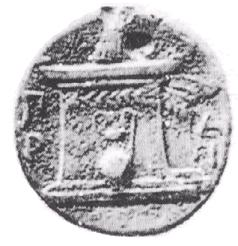
\includegraphics[scale=0.3]{images/logo}
\end{figure}
\vspace{-0.2in} 
\textbf{\gt \fontsize{14pt}{16.8pt} \bf \greektext{ΧΑΡΟΚΟΠΕΙΟ ΠΑΝΕΠΙΣΤΗΜΙΟ ΑΘΗΝΩΝ}\\}
\vspace{0.2in}
{\fontsize{12pt}{14.4pt}  
ΤΜΗΜΑ ΠΛΗΡΟΦΟΡΙΚΗΣ ΚΑΙ ΤΗΛΕΜΑΤΙΚΗΣ}
\vspace{1.3in}

{ \fontsize{12pt}{14.4pt}  \bf ΠΤΥΧΙΑΚΗ ΕΡΓΑΣΙΑ}
%
\vspace{0.7in}


% title assumed to be 3 lines long
{  \fontsize{16pt}{19.2pt} \bf Συλλογή και κατηγοριοποίηση δεδομένων κίνησης, μέσω κινητών τηλεφώνων, με στόχο την ανίχνευση δραστηριότητας\gt\\ }

\vspace{0.4in}

{ \fontsize{12pt}{14.4pt}  \bf Τραγοπούλου Σπυριδούλα }

\vspace{0.6in}

{\fontsize{12pt}{14.4pt}  
\begin{tabular}{cl}
Επιβλέποντες: & {\bf Βαρλάμης Ηρακλής},  Λέκτορας\\
& {\bf Τσερπές Κωνσταντίνος}, Λέκτορας\\
\end{tabular}}


\vspace{1.5in}


{\fontsize{12pt}{14.4pt}  \bf ΑΘΗΝΑ \\\vspace{0.2in} ΣΕΠΤΕΜΒΡΙΟΣ 2013\\}
\end{centering}

%%%%%%%%%%%%%%%%%%%%%%%%%%%%%%%%%%%%%%%%%%%%%%%%%%%%%%%%%%%%%%%%%%%%%%%%%%%%%%%%%

\begin{doublespacing}
\chapter*{Περίληψη}
\end{doublespacing}
\thispagestyle{empty}
\normalsize
\doublespacing
\paragraph[]{} Περίληψη. \\\\\\\\\\\\\\\\\\\\\\\\\
ΘΕΜΑΤΙΚΗ ΠΕΡΙΟΧΗ: \\
ΛΕΞΕΙΣ ΚΛΕΙΔΙΑ:  \\

\clearpage\newpage
%%%%%%%%%%%%%%%%%%%%%%%%%%%%%%%%%%%%%%%%%%%%%%%%%%%%%%%%%%%%%%%%%%%%%%%%%%%%%%%%%
\begin{doublespacing}
\chapter*{\lt Abstract}
\end{doublespacing}
\thispagestyle{empty}
\normalsize
\doublespacing
\paragraph[]{} \lt Abstract. \\\\\\\\\\\\\\\\\\\\\\\\\
SUBJECT AREA: \\
KEYWORDS:  \\
\gt
%%%%%%%%%%%%%%%%%%%%%%%%%%%%%%%%%%%%%%%%%%%%%%%%%%%%%%%%%%%%%%%%%%%%%%%%%%%%%%%%%

\chapter*{Ευχαριστίες}
\thispagestyle{empty}
\normalsize
\onehalfspacing
\paragraph[]{} Ευχαριστίες.
\clearpage\newpage

%%%%%%%%%%%%%%%%%%%%%%%%%%%%%%%%%%%%%%%%%%%%%%%%%%%%%%%%%%%%%%%%%%%%%%%%%%%%%%%%%
\pagestyle{fancy}
\begin{doublespacing}
%every chapter should be on the right side (odd page no.)
\tableofcontents
\clearpage\newpage
\listoffigures
\clearpage\newpage
\listoftables 
\end{doublespacing}
\clearpage


\chapter*{Πρόλογος}
\addcontentsline{toc}{chapter}{Πρόλογος}
\paragraph[]{} Πρόλογος.  
\onehalfspacing
%%%%%%%%%%%%%%%%%%%%%%%%%%%%%%%%%%%%%%%%%%%%%%%%%%%%%%%%%%%%%%%%%%%%%%%%%%%%%%%%%
%%%%%%%%%%%%%%%%%%%%%%%%%%%%%%%%%%%%%%%%%%%%%%%%%%%%%%%%%%%%%%%%%%%%%%%%%%%%%%%%%
\chapter[Εισαγωγή]{Εισαγωγή}
\gt Η τεχνολογία των ασύρματων επικοινωνιών και του \lt ubiquitous computing \gtκατακλύζουν την καθημερινότητα της σύγχρονης κοινωνίας. Τα ασύρματα δίκτυα καλύπτουν την μεγαλύτερη έκταση των αστικών κέντρων, ενώ ο αριθμός των χρηστών έξυπνων τηλεφώνων αυξάνεται καθημερινά. Τα \lt smartphones \gt παρέχουν εφαρμογές καταγραφής διάφορων μορφών δεδομένων κάνοντας χρήση ενσωματωμένων αισθητήρων, όπως \lt Bluetooth, GPS, \gt πυξίδα, φωτογραφική μηχανή κα μικρόφωνο. Αυτοί οι αισθητήρες, κάνοντας χρήση ασύρματων δικτύων μπορούν να ανιχνεύσουν την θέση και την κίνηση του χρήστη κατά τη διάρκεια χρήσης του κινητού τηλεφώνου. Κατά συνέπεια, η συλλογή δεδομένων κίνησης από την καθημερινότητα του χρήστη αποτελεί μια απλή διαδικασία, η οποία έχει ως στόχο με την ανάλυση των δεδομένων να διευκολύνει τις διάφορες δραστηριότητες του, παρακολουθώντας τον τρόπο ζωής του. Επιπλέον, η παρακολούθηση και ο έλεγχος της καθημερινής δραστηριότητας του ατόμου βρίσκουν εφαρμογή στην υγειονομική περίθαλψη, καθώς με αυτόν τον τρόπο μπορούν να διαγνωστούν σοβαρά προβλήματα υγείας ή ακόμα να εποπτευθούν ασθενείς που χρειάζονται μετεγχειρητική παρακολούθηση.
%%%%%%%%%%%%%%%%%%%%%%%%%%%%%%%%%%%%%%%%%%%%%%%%%%%%%%%%%%%%%%%%%%%%%%%%%%%%%%%%% 
\section[Σκοπός της πτυχιακής εργασίας]{Σκοπός της πτυχιακής εργασίας}
\gtΟι χρήστες έξυπνων κινητών τηλεφώνων χρησιμοποιούν στην καθημερινότητα τους, εφαρμογές που καταγράφουν δεδομένα (θέσης, δραστηριότητας, χρήσης), τα οποία μπορούν να χρησιμοποιηθούν εφόσον αναλυθούν. Σκοπός της παρούσας πτυχιακής εργασίας είναι η ανάπτυξη μιας εφαρμογής για έξυπνα τηλέφωνα, η οποία θα καταγράφει δεδομένα κίνησης, θα τα αναλύει και θα τα συνδυάζει με δεδομένα συγκοινωνιακού δικτύου με στόχο την ανίχνευση δραστηριότητας. 

\gtΗ εφαρμογή λειτουργεί σε κινητά με λειτουργικό σύστημα \lt Android,  \gt καταγράφει διαρκώς δεδομένα θέσης του χρήστη με χρήση \lt GPS \gt και τα επεξεργάζεται τοπικά κάνοντας χρήση τεχνικών εξόρυξης δεδομένων, προσδιορίζοντας τον τύπο κίνησης του χρήστη μέσα στη μέρα. Πιο συγκεκριμένα, η αναγνώριση της κίνησης υλοποιήθηκε με τη μέθοδο της κατηγοριοποίησης \lt(classification), \gt κάνοντας χρήση των αλγορίθμων κατηγοριοποίησης που παρέχει το λογισμικό \lt Weka, \gt όπως  ο \lt C4.5 (j48) \gt και ο \lt Random Forest. \gt Για την εκπαίδευση του συστήματος, χρησιμοποιήθηκαν δεδομένα εκπαίδευσης καταγεγραμμένα από την ίδια εφαρμογή.

%%%%%%%%%%%%%%%%%%%%%%%%%%%%%%%%%%%%%%%%%%%%%%%%%%%%%%%%%%%%%%%%%%%%%%%%%%%%%%%%%
\section[\lt{Smartphones} \gt{και Λειτουργικό Σύστημα} \lt{Android}]{\lt{Smartphones} \gt{και Λειτουργικό Σύστημα} \lt{Android}}

\subsection{\lt Smartphones\gt}
Με τον όρο έξυπνο τηλέφωνο \lt (smartphone) \gt αναφερόμαστε σε ένα κινητό τηλέφωνο βασισμένο σε ένα λειτουργικό σύστημα κινητής τηλεφωνίας με περισσότερη προηγμένη υπολογιστική ικανότητα και συνδεσιμότητα σε σχέση με ένα απλό κινητό τηλέφωνο.  Τα σύγχρονα \lt smartphones \gt αποτελούν πολυχρηστικές συσκευές καθώς περιλαμβάνουν λειτουργίες \lt media players, \gt ψηφιακές φωτογραφικές μηχανές, πλοήγηση \lt GPS, \gt οθόνες αφής υψηλής ανάλυσης και \lt web browsers \gt που εμφανίζουν τυποποιημένες ιστοσελίδες, καθώς και βελτιστοποιημένες ιστοσελίδες για κινητά. Η πρόσβαση σε δεδομένα υψηλής ταχύτητας παρέχεται μέσω \lt Wi-Fi \gt και μέσω ασύρματων ευρυζωνικών υπηρεσιών. Τα λειτουργικά συστήματα \lt (OS) \gt των κινητών τηλεφώνων που χρησιμοποιούνται από τα σύγχρονα smartphones περιλαμβάνουν το \lt Android \gt της \lt Google, \gt το \lt iOS \gt της \lt Apple, \gt το \lt Symbian \gt της \lt Nokia, \gt το \lt BlackBerry OS \gt της \lt RIM, \gt το \lt Firefox OS \gt της \lt Mozilla \gt και το \lt Ubuntu Phone \gt της \lt Canonical Ltd's\gt.\cite{smartphone}

\subsection*{\gtΑισθητήρες \lt Smartphones\gt}
\subsubsection*{\lt Global Positioning System (GPS)\gt}
Το \lt GPS (Global Positioning System), \gtΠαγκόσμιο Σύστημα Θεσιθεσίας είναι ένα παγκόσμιο σύστημα εντοπισμού θέσης, το οποίο βασίζεται σε εικοσιτέσσερις δορυφόρους της Γης, οι οποίοι διαθέτουν ειδικές συσκευές ονομάζονται δέκτες \lt GPS. \gt Οι δέκτες αυτοί παρέχουν ακριβείς πληροφορίες για τη θέση ενός σημείου, το υψόμετρό του, την ταχύτητα και την κατεύθυνση της κίνησης του.  Το \lt GPS \gt παρέχει πληροφορίες τοποθεσίας και χρόνου σε όλες τις καιρικές συνθήκες, οπουδήποτε πάνω ή κοντά στη Γη, όπου υπάρχει ανεμπόδιστη οπτική επαφή με τέσσερις ή περισσότερους δορυφόρους \lt GPS. \gt Συντηρείται από την κυβέρνηση των Ηνωμένων Πολιτειών και είναι ελεύθερα προσβάσιμο με ένα δέκτη \lt GPS. 
\gt Το \lt GPS \gt δημιουργήθηκε αναπτύχθηκε το 1973  από το Υπουργείο Άμυνας των ΗΠΑ με σκοπό να ξεπεράσει τους περιορισμούς των προηγούμενων συστημάτων πλοήγησης . Αρχικά ονομάστηκε \lt "NAVSTAR GPS" (Navigation Signal Timing and Ranging Global Positioning System) \gt και τέθηκε σε πλήρη λειτουργία το 1994. \cite{gps_wiki} Για τον προσδιορισμό της θέσης του χρήστη με γεωγραφικό μήκος \lt (longitude) \gt και γεωγραφικό πλάτος \lt (latitude) \gt απαιτείται σύνδεση σε τρεις δορυφόρους, ενώ για τον προσδιορισμό του υψόμετρου απαιτούνται τέσσερις δορυφόροι.

Η πλειοψηφία των δεκτών \lt GPS \gt βρίσκονται σε κινητά τηλέφωνα, με ποικίλους βαθμούς κάλυψης και προσβασιμότητας των χρηστών. Στα περισσότερα \lt smartphones \gt υπάρχει διαθέσιμο λογισμικό πλοήγησης, καθώς και σε ορισμένα τηλέφωνα που διαθέτουν \lt Java \gt που τους επιτρέπει να χρησιμοποιούν εσωτερικό ή εξωτερικό δέκτη \lt GPS. \gt Ακόμα, μερικά κινητά τηλέφωνα χρησιμοποιούν \lt A-GPS (assisted GPS), \gt  το οποίο όμως υπολειτουργεί όταν βρίσκεται εκτός του δικτύου κινητής τηλεφωνίας. Παράλληλα, μερικά άλλα χρησιμοποιούν ένα υβριδικό σύστημα εντοπισμού θέσης που μπορούν να χρησιμοποιήσουν άλλα σήματα, όταν τα σήματα \lt GPS \gt είναι ανεπαρκή.\cite{gps_dev}

Στα κινητά τηλέφωνα, η θέση μπορεί να οριστεί είτε με χρήση \lt GPS, \gt είτε με τον τριγωνισμό της απόστασης από την κεραία της κινητής τηλεφωνίας ή το ασύρματο δίκτυο \lt (Wi-Fi) \gt που χρησιμοποιεί ο χρήστης, είτε θεωρώντας ως τοποθεσία του χρήστη την κεραία της κινητής τηλεφωνίας ή του ασύρματου δικτύου. Τα \lt smartphones \gt έχουν τη δυνατότητα να επιλέγουν κάθε φορά τον βέλτιστο τρόπο για τον ορισμό της θέσης του χρήστη.\cite{sensors}

\subsubsection*{\gt Επιταχυνσιόμετρο \lt (accelerometer)\gt}
Το επιταχυνσιόμετρο είναι μια συσκευή που μετρά την επιτάχυνση. Η επιτάχυνση που μετράει δεν είναι απαραιτήτως η επιτάχυνση με βάση τις συντεταγμένες (ρυθμός μεταβολής της ταχύτητας). Αντίθετα, το επιταχυνσιόμετρο υπολογίζει την επιτάχυνση που συνδέεται με το φαινόμενο του βάρους οποιασδήποτε μάζας σε αδράνεια σε σχέση με τη διάταξη της συσκευής.

Μερικά \lt smartphones, \gt περιέχουν επιταχυνσιόμετρα για τον έλεγχο της διεπαφής χρήστη. Συχνά το επιταχυνσιόμετρο χρησιμοποιείται για να παρουσιάσει θέα στο γύρω τοπίο ή πορτρέτο της οθόνης της συσκευής, με βάση την διάταξη της συσκευής. Η 5η και 6η γενιά \lt Apple iPod Nano \gt διαθέτει ένα ενσωματωμένο επιταχυνσιόμετρο και μια εφαρμογή  που ονομάζεται \lt Fitness \gt και μπορεί να χρησιμοποιηθεί για να καταγράψει τα βήματα κατά το περπάτημα ή το τρέξιμο.\cite{accelerometer}

\subsubsection*{\gt Μαγνητόμετρο \lt (magnetometer)\gt}

Το μαγνητόμετρο είναι ένα όργανο μέτρησης της δύναμης και σε ορισμένες περιπτώσεις, της κατεύθυνσης των μαγνητικών πεδίων. Πολλά \lt smartphones \gt διαθέτουν μαγνητόμετρα και παρέχουν εφαρμογές που λειτουργούν ως πυξίδες. Άλλες συσκευές τηλεφώνων, χρησιμοποιούν μαγνητόμετρα τριών αξόνων, τα οποία δεν είναι ευαίσθητα στον προσανατολισμό ή την ανύψωση της συσκευής. Ερευνητές στην \lt Deutsche Telekom \gt έχουν χρησιμοποιήσει μαγνητόμετρα ενσωματωμένα σε κινητές συσκευές για να επιτρέπουν \lt 3D \gt αλληλεπίδραση του χρήστη χωρίς αφή. Η διεπαφή που δημιούργησαν, ονομάζεται \lt MagiTact \gt και παρακολουθεί τις αλλαγές στο μαγνητικό πεδίο γύρω από ένα κινητό τηλέφωνο για να εντοπίσει τις διάφορες χειρονομίες από ένα χέρι που κρατάει ή φοράει ένα μαγνήτη.\cite{magnetometer}

\subsection{\gt Λειτουργικό Σύστημα \lt Android\gt}
Το \lt Android \gt είναι λειτουργικό σύστημα το οποίο τρέχει τον πυρήνα του λειτουργικού \lt Linux \gt και έχει σχεδιαστεί για κινητές συσκευές με οθόνη αφής όπως \lt smartphones \gt και \lt tablets. \gt Αρχικά αναπτύχθηκε από την \lt Google \gt και αργότερα από την \lt Open Handset Alliance. \gt Το πρώτο κινητό τηλέφωνο με \lt Android \gt κυκλοφόρησε τον Οκτώβριο του 2008.  Η \lt Google \gt δημοσίευσε το μεγαλύτερο μέρος του κώδικα του \lt Android \gt υπό τους όρους της \lt Apache License, \gt μιας ελεύθερης άδειας λογισμικού. Αυτό σημαίνει ότι το \lt Android \gt μπορεί  να τροποποιηθεί και να διανεμηθεί ελεύθερα από τους κατασκευαστές συσκευών και τους προγραμματιστές. Επιπλέον, το \lt Android \gt διαθέτει μια μεγάλη κοινότητα προγραμματιστών που αναπτύσσουν εφαρμογές οι οποίες επεκτείνουν τη λειτουργικότητα των συσκευών, γραμμένες σε μια προσαρμοσμένη έκδοση της γλώσσας προγραμματισμού \lt Java \gt για \lt Android.\gt

Αυτοί οι παράγοντες συνέβαλαν στο να γίνει το \lt Android \gt το πιο ευρέως χρησιμοποιούμενο λειτουργικό σύστημα για \lt smartphone \gt και το λογισμικό που επιλέγουν οι περισσότερες εταιρείες λογισμικού για συσκευές υψηλής τεχνολογίας, καθώς έχει χαμηλό κόστος, είναι προσαρμόσιμο και ελαφρύ και δεν απαιτείται ανάπτυξη λογισμικού από το μηδέν. Αυτό έχει ως αποτέλεσμα, παρά το γεγονός ότι αρχικά σχεδιάστηκε για \lt smartphones \gt και \lt tablets, \gt να έχουν δημιουργηθεί εφαρμογές \lt Android \gt για τηλεοράσεις, κονσόλες παιχνιδιών και ψηφιακές κάμερες.\cite{android}

\subsubsection{Εκδόσεις \lt Android\gt}
Η πρώτη \lt beta \gtέκδοση \lt Android \gtκυκλοφόρησε στις 5 Νοεμβρίου 2007. Από τότε έχουν κυκλοφορήσει πολλές εκδόσεις και έχουν γίνει ενημερώσεις οι οποίες περιγράφονται σε κάθε έκδοση με έναν αριθμό  που ονομάζεται \lt API Level \gtκαι προσδιορίζει το \lt API framework \gtπου υποστηρίζεται. Στον πίνακα \ref{fig:androidVer} παρουσιάζονται όλες οι εκδόσεις \lt Android \gtπου έχουν κυκλοφορήσει, με το  \lt API Level \gtπου υποστηρίζουν\cite{android_versions}.
\begin{figure}[H]
\centering
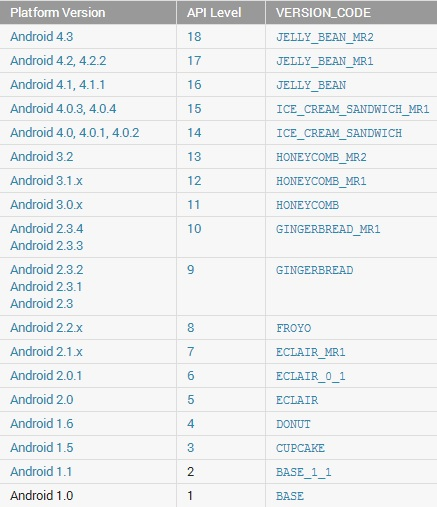
\includegraphics{images/android_versions}
\caption{Οι εκδόσεις \lt Android \gt που έχουν κυκλοφορήσει.}
\label{fig:androidVer}
\end{figure}
Τα στατιστικά στοιχεία χρήσης των εκδόσεων \lt Android\gt, τα οποία έχουν καταγραφεί μέχρι και την 1η Αυγούστου 2013, παρουσιάζονται παρακάτω. Οι εκδόσεις που κατέχουν ποσοστό χρήσης μικρότερο από 0,1\% δεν φαίνονται στο σχήμα.
\begin{figure}[H]
\centering
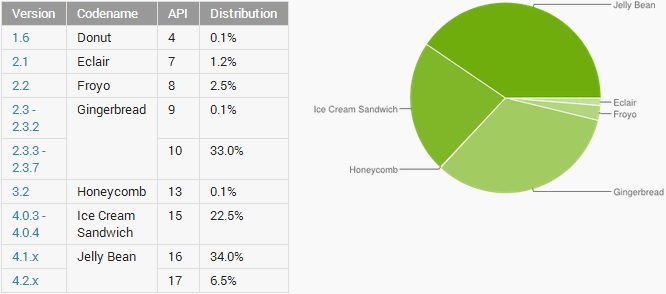
\includegraphics{images/distribution}
\caption{Η κατανομή χρήσης των εκδόσεων \lt Android.\gt}
\end{figure}
\subsubsection{Αρχιτεκτονική του \lt Android\gt}
Το λειτουργικό σύστημα \lt Android \gt αποτελείται από τέσσερα βασικά επίπεδα, τα οποία χωρίζονται σε πέντε τμήματα, όπως φαίνεται στο Σχήμα \ref{fig:androidArc}\cite{Lee:2011}.
\begin{itemize}
\item\emph{Πυρήνας \lt Linux\gt} - Αποτελεί τον πυρήνα στον οποίο είναι βασισμένο το \lt Android\gt. Αυτό το επίπεδο, περιλαμβάνει όλους τους χαμηλού επιπέδου οδηγούς συσκευών για όλα τα \lt hardware \gtεξαρτήματα της συσκευής \lt Android\gt.
\item\emph{Βιβλιοθήκες \lt (Libraries)\gt} - Περιλαμβάνει τον κώδικα ο οποίος παρέχει τα βασικά χαρακτηριστικά του \lt Android. \gtΓια παράδειγμα, η βιβλιοθήκη \lt WebKit \gtπαρέχει λειτουργικότητα για περιήγηση στον ιστό.
\item\emph{\lt Android Runtime\gt} - Στο ίδιο επίπεδο με τις βιβλιοθήκες, το \lt Android Runtime \gtδιαθέτει βιβλιοθήκες πυρήνα που επιτρέπουν στους προγραμματιστές να αναπτύσσουν εφαρμογές \lt Android \gtκάνοντας χρήσης της γλώσσας προγραμματισμού \lt Java\gt. Ακόμα, διαθέτει στην εικονική μηχανή \lt Dalvik, \gtη οποία επιτρέπει σε κάθε εφαρμογή να τρέχει σε ξεχωριστή διεργασία.Η Dalvik είναι μια εικονική μηχανή σχεδιασμένη για Android και βελτιστοποιημένη για να λειτουργεί σε κινητές συσκευές με μπαταρία και και περιορισμένη μνήμη και επεξεργαστική ισχύ. 
\item\emph{\lt Framework \gtΕφαρμογών} - Προσφέρει τις ποικίλες δυνατότητες του λειτουργικού \lt Android \gtστους προγραμματιστές εφαρμογών, ώστε να μπορούν να τις χρησιμοποιήσουν στις εφαρμογές που δημιουργούν. 
\item\emph{Εφαρμογές} - Αποτελεί το υψηλότερο επίπεδο του λειτουργικού και διαθέτει όλες τις εφαρμογές που τρέχουν στη συσκευή όπως το τηλέφωνο, την διαχείριση επαφών και τον περιηγητή ιστού.
\end{itemize}
\begin{figure}[H]
\centering
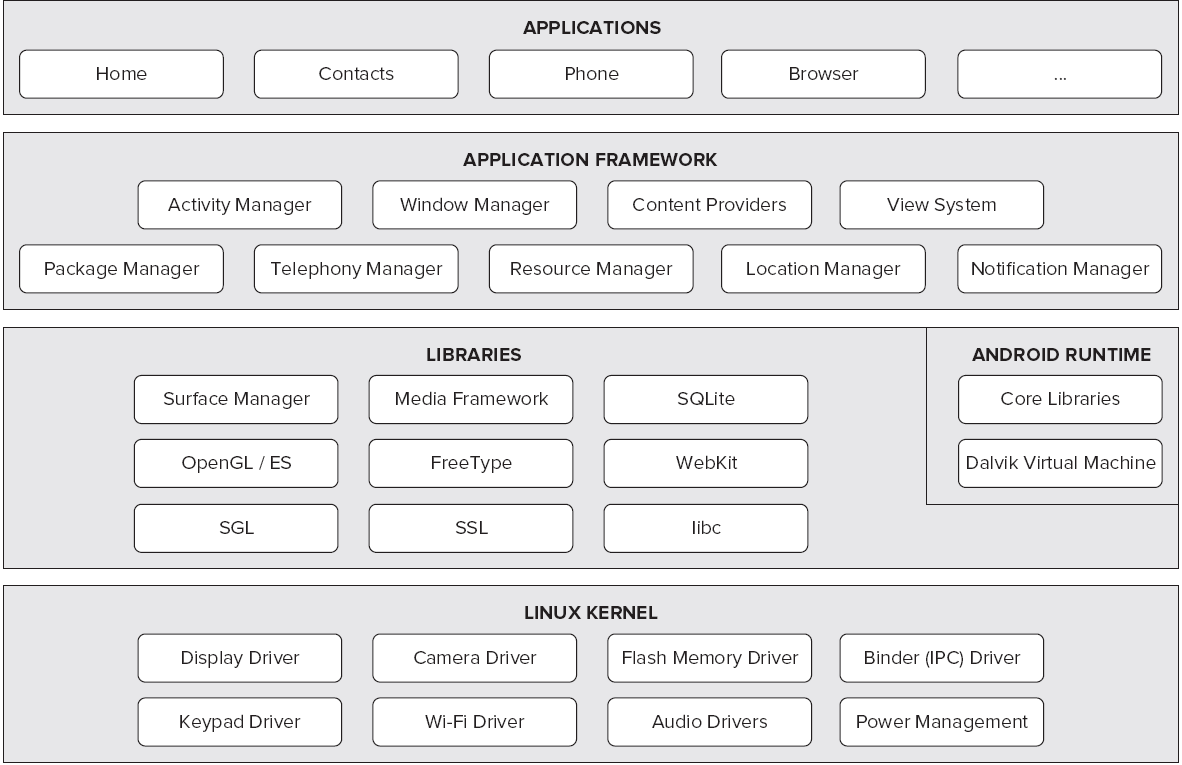
\includegraphics[height=10cm]{images/android_arc}
\caption{Η αρχιτεκτονική του λειτουργικού συστήματος \lt Android\gt}
\label{fig:androidArc}
\end{figure}
\subsubsection{Χαρακτηριστικά του \lt Android\gt}
Λόγω του ότι ότι το \lt Android \gtαποτελεί λειτουργικό σύστημα ανοιχτού κώδικα και είναι διαθέσιμο για οποιαδήποτε τροποποίηση, δεν περιλαμβάνει καθορισμένες ρυθμίσεις υλικού και λογισμικού. Παρόλα αυτά, υποστηρίζει από μόνο του τις  λειτουργίες που περιγράφονται παρακάτω\cite{Lee:2011}.
\begin{itemize}
\item\emph{Αποθήκευση Δεδομένων} - Χρήση της \lt SQLite \gt, μιας ελαφριάς βάσης δεδομένων για τις ανάγκες αποθήκευσης.
\item\emph{Συνδεσιμότητα} - Υποστηρίζει τεχνολογίες συνδεσιμότητας \lt GSM/EDGE, CDMA, IDEN, EV-DO, UMTS, Bluetooth, LTE, WiMAX \gt και \lt Wi-Fi.\gt
\item\emph{Υπηρεσίες Μηνυμάτων} - Υποστηρίζει αποστολή και λήψη \lt SMS \gtκαι \lt MMS.\gt
\item\emph{Περιήγηση στον Ιστό} - Για την περιήγηση στον ιστό διαθέτει φυλλομετρητή βασισμένο στην ανοιχτή τεχνολογία \lt WebKit.\gt
\item\emph{Υποστήριξη Πολυμέσων} - Παρέχει υποστήριξη για τις ακόλουθες μορφές πολυμέσων: \lt H.263, H.264 (\gt σε \lt 3GP \gt ή \lt MP4container), MPEG-4 SP, AMR, AMR-WB, AAC, HE-AAC, MP3, MIDI, OGG Vorbis, WAV, JPEG, PNG, GIF, BMP. \gt 
\item\emph{Υποστήριξη υλικού} - Υποστηρίζει κάμερες στατικής ή κινούμενης εικόνας, οθόνες αφής, \lt GPS, \gt αισθητήρες επιτάχυνσης, μαγνητόμετρα, καθώς και proximity sensors.                                                            
\item\emph{\lt Multitasking\gt} - Υποστηρίζει \lt multitasking \gtεφαρμογές.
\end{itemize}

Οι περισσότερες λειτουργίες του τηλεφώνου τρέχουν σαν εφαρμογές πάνω στο ενδιάμεσο λογισμικό \lt (middleware) \gt που διαθέτει. Το ενδιάμεσο λογισμικό είναι γραμμένο σε \lt Java \gt και \lt C/C++. \gt Οι εφαρμογές που τρέχουν σε \lt Android \gt είναι γραμμένες σε \lt Java \gt και μεταγλωττίζονται σε προσαρμοσμένο πηγαίο κώδικα που ονομάζεται  \lt Dalvik EXecutable (DEX) \gt και εκτελούνται στην εικονική μηχανή \lt Dalvik VM, \gt η οποία είναι σχεδιασμένη για χρήση σε φορητές συσκευές. Οι εφαρμογές επικοινωνούν με τον μηχανισμό \lt binder IPC, \gt o  οποίος παρέχει διαφανή ανταλλαγή μηνυμάτων με χρήση δεμάτων.\cite{taintdroid}

Οι εφαρμογές \lt Android \gt αναπτύσσονται στη γλώσσα \lt Java \gt χρησιμοποιώντας το \lt Android Software Development Kit (SDK). \gt Το \lt SDK \gt περιλαμβάνει ένα ολοκληρωμένο σύνολο εργαλείων ανάπτυξης, όπως πρόγραμμα εντοπισμού σφαλμάτων \lt(debugger), \gt βιβλιοθήκες λογισμικού, \lt emulator \gt κινητού τηλεφώνου που  βασίζεται σε \lt QEMU, documentation, \gt δείγματα κώδικα και \lt tutorials. \gt Το επίσημο περιβάλλον ανάπτυξης για εφαρμογές \lt Android \gt είναι το \lt Eclipse (IDE)  \gt κάνοντας χρήση του \lt Android Development Tools (ADT) plugin. \gt \cite{android}

Ακόμα, το περιβάλλον προγραμματισμού \lt Eclipse \gt επιτρέπει την ενσωμάτωση εργαλείων και τεχνικών εξόρυξης δεδομένων χρησιμοποιώντας το \lt API \gt του \lt Weka. \gt Το \lt Weka \gt προσφέρει ένα πακέτο κλάσεων για προγραμματιστές που επιτρέπει την διαχείριση και  την προεπεξεργασία  δεδομένων \lt (preprocessing), \gt αλγορίθμους κατηγοριοποίησης \lt (classification) \gt και συσταδοποίησης \lt (clustering) \gt και την αξιολόγηση των επιδόσεων τους \lt (evaluation). \gt Έτσι, συμπεριλαμβάνοντας το πακέτο των κλάσεων του \lt Weka \gt και μέσω κώδικα \lt Java \gt είναι δυνατή η χρήση τεχνικών εξόρυξης γνώσης σε εφαρμογές \lt Android.\gt  \cite{wekawithjava}  

%%%%%%%%%%%%%%%%%%%%%%%%%%%%%%%%%%%%%%%%%%%%%%%%%%%%%%%%%%%%%%%%%%%%%%%%%%%%%%%%%
\section[Εξόρυξη Δεδομένων και Εξόρυξη Δεδομένων σε Κινητές Συσκευές]{Εξόρυξη Δεδομένων και Εξόρυξη Δεδομένων σε Κινητές Συσκευές}
\subsection{Εξόρυξη Δεδομένων \lt (Data Mining)\gt}
Με τον όρο \emph{εξόρυξη δεδομένων} αναφερόμαστε στη διαδικασία επιλογής, εξερεύνησης και μοντελοποίησης μεγάλου όγκου δεδομένων, με σκοπό  την εξαγωγή συμπερασμάτων τα οποία είναι αρχικά άγνωστα, ώστε να προκύψουν σαφή και χρήσιμα αποτελέσματα για τον χρήστη της βάσης δεδομένων\cite{Giudici:2009}.

Η ανακάλυψη γνώσης από μια βάση δεδομένων \lt (KDD - Knowledge Discovery from Database)\gt, αναφέρεται σε ολόκληρη τη διαδικασία ανακάλυψης χρήσιμης πληροφορίας από μεγάλα σύνολα δεδομένων\cite{vazirgiannis2005halkidi}. Η εξόρυξη δεδομένων αποτελεί το βήμα της \lt KDD \gt διαδικασίας, στο οποίο οι αλγόριθμοι εκμάθησης εφαρμόζονται στα δεδομένα\cite{Giudici:2009}.

Η διαδικασία \lt \emph{KDD} \gt είναι μια διαλογική και επαναληπτική διαδικασία που αποτελείται από μια σειρά από τα ακόλουθα βήματα (Σχήμα\ref{fig:KDDprocess}) \cite{vazirgiannis2005halkidi}.
\begin{figure}[H]
\centering
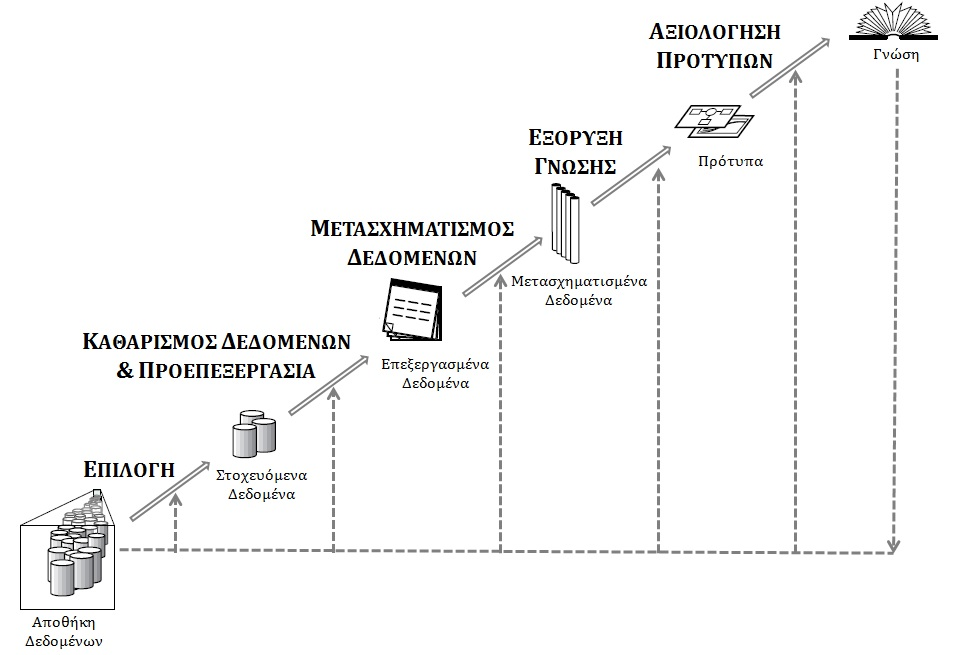
\includegraphics[height=12cm]{images/kdd_process}
\caption{Η διαδικασία ανακάλυψης γνώσης από μια βάση δεδομένων \lt (KDD) \gt}
\label{fig:KDDprocess}
\end{figure}
\begin{enumerate}
  \item \emph{Ανάπτυξη και κατανόηση} της περιοχής της εφαρμογής, της υπάρχουσας γνώσης στον τομέα έρευνας και τους τελικούς στόχους.
  \item \emph{Ολοκλήρωση των δεδομένων}, συνδυάζοντας πολλαπλές πηγές δεδομένων ώστε να καθοριστεί το σύνολο στο οποίο τελικά η διαδικασία εξόρυξης πρόκειται να εφαρμοστεί.
  \item \emph{Δημιουργία του στόχου – συνόλου δεδομένων}, επιλέγοντας το σύνολο δεδομένων (μεταβλητές, δείγματα δεδομένων) στο οποίο η διαδικασία εξόρυξης πρόκειται να εκτελεστεί.
  \item \emph{Καθαρισμός και προεπεξεργασία δεδομένων}, εφαρμόζοντας βασικές διαδικασίες όπως η αφαίρεση θορύβου, η συλλογή των απαραίτητων πληροφοριών για τη διαμόρφωση ή τη μέτρηση του θορύβου, η απόφαση σχετικά με τις στρατηγικές διαχείρισης των ελλειπόντων πεδίων δεδομένων.
  \item \emph{Μετασχηματισμός των δεδομένων}. Τα δεδομένα μετασχηματίζονται σε μορφές κατάλληλες για εξόρυξη, κάνοντας χρήση μεθόδων μείωσης διαστάσεων για τη μείωση των υπό εξέταση μεταβλητών ή την εύρεση κατάλληλης αντιπροσώπευσης των δεδομένων χωρίς μεταβλητές.
  \item \emph{Επιλογή των στόχων και των αλγορίθμων εξόρυξης δεδομένων}. Σε αυτό το βήμα αποφασίζεται ο στόχος της \lt KDD\gt διαδικασίας, επιλέγοντας τους στόχους εξόρυξης δεδομένων που πρέπει να επιτευχθούν. Ακόμα, επιλέγονται οι μέθοδοι εξόρυξης δεδομένων που θα χρησιμοποιηθούν, λαμβάνοντας υπόψη τις απαιτήσεις και τα γενικά κριτήρια της \lt KDD \gtδιαδικασίας.
  \item \emph{Εξόρυξη δεδομένων}, εφαρμόζοντας ευφυείς μεθόδους με στόχο την εύρεση προτύπων γνώσης. Τα πρότυπα μπορεί να είναι κανόνες κατηγοριοποίησης, δέντρα, παλινδρόμηση, συσταδοποίηση, κτλ.
  \item \emph{Αξιολόγηση των προτύπων}. Τα πρότυπα που προέκυψαν από την εξόρυξη δεδομένων αξιολογούνται με κάποια μέτρα, προκειμένου να προσδιοριστούν τα πρότυπα που αντιπροσωπεύουν καλύτερα την εξαγόμενη γνώση.
  \item \emph{Σταθεροποίηση και παρουσίαση της γνώσης}, ενσωματώνοντας τη γνώση στο σύστημα ή απεικονίζοντας την χρησιμοποιώντας τεχνικές αντιπροσώπευσης γνώσης, ώστε να μπορεί να παρουσιαστεί η εξορυγμένη γνώση στον χρήστη.
\end{enumerate}
\subsubsection{Μέθοδοι Εξόρυξης Δεδομένων}
Η εξόρυξη δεδομένων έχει ως βασικό στόχο την εφαρμογή τεχνικών περιγραφής και πρόβλεψης σε μεγάλα σύνολα δεδομένων. Η \emph{πρόβλεψη} έχει ως στόχο την πρόβλεψη της συμπεριφοράς κάποιων μεταβλητών που παρουσιάζουν ενδιαφέρον και οι οποίες βασίζονται στην συμπεριφορά άλλων μεταβλητών. Η \emph{περιγραφή} στοχεύει στην ανακάλυψη προτύπων και αναπαριστά τα δεδομένα μιας πολύπλοκης βάσης δεδομένων με κατανοητό και αξιοποιήσιμο τρόπο. Όλες οι υπάρχουσες μέθοδοι εξόρυξης δεδομένων έχουν ως βασικό στόχο να προσδιορίσουν και να περιγράψουν τα πρότυπα γνώσης που εξάγονται από ένα σύνολο δεδομένων. Οι κυριότερες μέθοδοι εξόρυξης δεδομένων περιγράφονται παρακάτω.
\begin{itemize}
 \item \emph{Κατηγοριοποίηση (\lt Classification).\gt} Αποτελεί μια από τις βασικές εργασίες εξόρυξης δεδομένων. Βασίζεται στην εξέταση των χαρακτηριστικών ενός μη-κατηγοριοποιημένου αντικειμένου, το οποίο με βάση αυτά τα χαρακτηριστικά αντιστοιχίζεται σε κάποια από τις κατηγορίες που έχουν προκαθοριστεί. Η βασική εργασία κατηγοριοποίησης, είναι η δημιουργία ενός μοντέλου το οποίο θα μπορούσε να εφαρμοστεί για να κατηγοριοποιεί μη-κατηγοριοποιημένα δεδομένα. Χρησιμοποιεί ένα σύνολο κατηγοριοποιημένων δεδομένων για την εκπαίδευση του μοντέλου και απαιτεί έναν καλά καθορισμένο ορισμό των κατηγοριών. Οι αλγόριθμοι κατηγοριοποίησης διακρίνονται σε δυο βασικές κατηγορίες τεχνικών, τα Δέντρα Απόφασης (\lt Decision Trees) \gt και τα Νευρωνικά Δίκτυα (\lt Neutral Networks)\gt.
 \item \emph{Συσταδοποίηση (\lt Clustering).\gt} Είναι η διαδικασία καταμερισμού ετερογενών δεδομένων σε ένα σύνολο περισσότερων ετερογενών συστάδων. Σε αντίθεση με την κατηγοριοποίηση, η συσταδοποίηση δεν βασίζεται σε προκαθορισμένες κατηγορίες. Οι εγγραφές των δεδομένων ομαδοποιούνται σε σύνολα με βάση την ομοιότητα που παρουσιάζουν μεταξύ τους.
\item \emph{Κανόνες Συσχέτισης (\lt Association Rules).\gt} Οι κανόνες συσχέτισης στοχεύουν στην ανακάλυψη κρυμμένων συσχετίσεων μεταξύ των γνωρισμάτων ενός συνόλου δεδομένων. Παρέχουν έναν συνοπτικό τρόπο για να εκφραστούν οι ενδεχομένως χρήσιμες πληροφορίες και να γίνουν κατανοητές από τους τελικούς χρήστες.
\item \emph{Πρότυπα ακολουθιών (\lt Sequential Patterns).\gt} Η εξόρυξη πρότυπων ακολουθιών αναφέρεται στην ανίχνευση των συχνά εμφανιζόμενων προτύπων σχετικών με τον χρόνο ή άλλες ακολουθίες. Οι περισσότερες έρευνες στα πρότυπα ακολουθιών επικεντρώνονται σε συμβολικά πρότυπα. 
\item \emph{Παλινδρόμηση (\lt Regression).\gt} Αναφέρεται στην εκμάθηση μιας λειτουργίας που εκχωρεί τα δεδομένα σε μια μεταβλητή πρόβλεψης, η οποία παίρνει πραγματικές τιμές.
\end{itemize}
\subsection{Εξόρυξη Δεδομένων σε Κινητές Συσκευές (\lt Mobile Data Mining)\gt}
Ο στόχος της εξόρυξης γνώσης σε κινητές συσκευές (\lt mobile data mining) \gtείναι να παρέχει προηγμένες τεχνικές για την ανάλυση και την παρακολούθηση δεδομένων που καταγράφονται μέσω κινητών συσκευών\cite{mobmining2010talia}.

Η εξόρυξη δεδομένων σε κινητές συσκευές, έχει να αντιμετωπίσει τα τυπικά ζητήματα της εξόρυξης δεδομένων σε ένα κατανεμημένο περιβάλλον ενώ ταυτόχρονα και τους τεχνολογικούς περιορισμούς ενός κινητού τηλεφώνου, όπως δίκτυα με χαμηλό \lt bandwidth, \gtπεριορισμένη χωρητικότητα αποθήκευσης, μικρή ισχύς μπαταρίας, αργούς επεξεργαστές και μικρές οθόνες για την απεικόνιση των αποτελεσμάτων\cite{Pittie:2003}.

Ο τομέας της εξόρυξης δεδομένων σε κινητές συσκευές περιλαμβάνει διάφορα σενάρια εφαρμογών, στις οποίες ένα κινητό τηλέφωνο μπορεί να καταγράφει δεδομένα, να τα αναλύει, να αποτελεί τον \lt client \gt ενός απομακρυσμένου \lt server \gtπου υλοποιεί την εξόρυξη δεδομένων ή να υλοποιεί τον συνδυασμό αυτών των λειτουργιών. Πιο συγκεκριμένα, μπορούμε να διακρίνουμε τρία βασικά σενάρια για την εξόρυξη δεδομένων σε κινητές συσκευές\cite{mobmining2010talia}.
\begin{enumerate}
\itemΗ κινητή συσκευή χρησιμοποιείται σαν τερματικό για την πρόσβαση σε έναν απομακρυσμένο \lt server \gtο οποίος παρέχει υπηρεσίες εξόρυξης δεδομένων. Ο \lt server \gtαναλύει τα δεδομένα που είναι αποθηκευμένα σε μια τοπική ή κατανεμημένη βάση δεδομένων και στέλνει τα αποτελέσματα της διαδικασίας εξόρυξης στην συσκευή για να τα απεικονίσει.
\itemΤα δεδομένα που καταγράφηκαν μέσω μιας κινητής συσκευής, αποστέλλονται σε έναν απομακρυσμένο \lt server \gtκαι αποθηκεύονται σε μια τοπική βάση δεδομένων. Τα δεδομένα αναλύονται κάνοντας χρήση συγκεκριμένων αλγορίθμων εξόρυξης δεδομένων και τα αποτελέσματα χρησιμοποιούνται για να ληφθούν αποφάσεις για κάποιο συγκεκριμένο σκοπό.
\itemΗ ανάλυση των δεδομένων υλοποιείται στις κινητές συσκευές. Βέβαια λόγω της μειωμένης επεξεργαστικής ισχύος και χωρητικότητας των σύγχρονων συσκευών, δεν είναι πάντα εφικτή η υλοποίηση όλων των αλγορίθμων εξόρυξης δεδομένων σε μια κινητή συσκευή. Ωστόσο, κάποια βήματα της διαδικασίας εξόρυξης, όπως η επιλογή και η προεπεξεργασία των δεδομένων μπορούν να εκτελεστούν σε μια τέτοια συσκευή, καθώς επίσης και μερικοί αλγόριθμοι εξόρυξης γνώσης που δεν απαιτούν μεγάλη επεξεργαστική ισχύ. 
\end{enumerate}

Μια πιο σύγχρονη προσέγγιση εξόρυξης δεδομένων σε κινητές συσκευές παρουσιάζουν οι \lt Steinbauer \gtκαι συν.\cite{SteinbauerKK13}, η οποία βασίζεται σε τεχνολογία \lt cloud. \gtΟ στόχος τους είναι να παρέχουν εργαλεία και τεχνικές για την ανάλυση δεδομένων κοινωνικών δικτύων σε σχεδόν πραγματικό χρόνο. Τα δεδομένα παράγονται και καταγράφονται από τους αισθητήρες της κινητής συσκευής και έπειτα αποστέλλονται  σε ένα δυναμικό μοντέλο \lt cloud \gtγια περαιτέρω επεξεργασία.
%%%%%%%%%%%%%%%%%%%%%%%%%%%%%%%%%%%%%%%%%%%%%%%%%%%%%%%%%%%%%%%%%%%%%%%%%%%%%%%%%
%%%%%%%%%%%%%%%%%%%%%%%%%%%%%%%%%%%%%%%%%%%%%%%%%%%%%%%%%%%%%%%%%%%%%%%%%%%%%%%%%
\chapter[Θεωρητικό Υπόβαθρο]{Θεωρητικό Υπόβαθρο}
\label{Chapter4}
%%%%%%%%%%%%%%%%%%%%%%%%%%%%%%%%%%%%%%%%%%%%%%%%%%%%%%%%%%%%%%%%%%%%%%%%%%%%%%%%%
\section[Εφαρμογές Δεδομένων Κίνησης]{Εφαρμογές Δεδομένων Κίνησης}
Παρακάτω παρουσιάζονται μερικές υπάρχουσες εφαρμογές για \lt Android \gt οι οποίες χρησιμοποιούν δεδομένα θέσης για να καταγράψουν την δραστηριότητα του χρήστη.
\subsection*{\lt My Tracks\gt }

Η εφαρμογή \lt My Tracks \gt της \lt Google \gt καταγράφει  τη διαδρομή, την ταχύτητα, την απόσταση και το υψόμετρο του χρήστη καθώς περπατάει, τρέχει, κάνει ποδήλατο ή οποιαδήποτε άλλη υπαίθρια δραστηριότητα.
\begin{figure}[H]
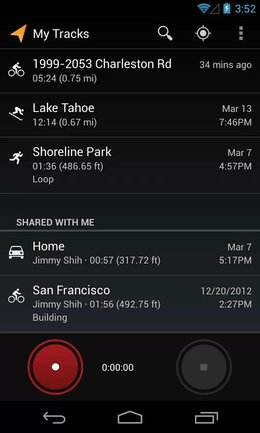
\includegraphics[height=8cm]{images/mt1}
\hspace{0.4in}
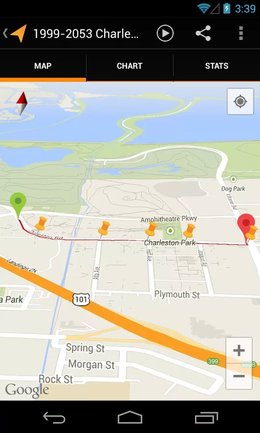
\includegraphics[height=8cm]{images/mt2}
\hspace{0.4in}
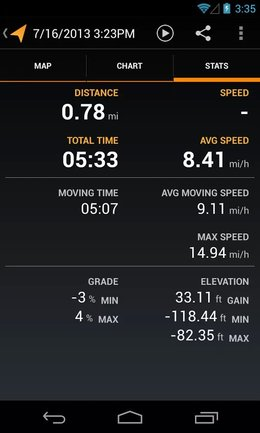
\includegraphics[height=8cm]{images/mt3}
\caption{Στιγμιότυπα χρήσης της εφαρμογής \lt MyTracks \gt}
\end{figure}
Ενώ καταγράφει δεδομένα, επιτρέπει στον χρήστη να δει τα δεδομένα κίνησης του, να χαρακτηρίσει την κίνηση που κάνει εκείνη τη στιγμή, ενώ ταυτόχρονα ακούει ανακοινώσεις για την πρόοδο των επιδόσεων του. Επίσης, εμφανίζει γραφήματα για την μεταβολή της ταχύτητας και του υψομέτρου σε προκαθορισμένες διαδρομές. Χρησιμοποιεί \lt GPS \gt για να καταγράψει γεωγραφικά δεδομένα και στατιστικά ταχύτητας αλλά και εξωτερικούς βιομετρικούς αισθητήρες \lt (Zephyr HxM, Polar WearLink, ANT+) \gt για να καταγράψει τον καρδιακό ρυθμό και την ταχύτητα. 

\subsection*{\lt Nike+ Running\gt }
Η εφαρμογή \lt Nike+ Running  \gt της \lt Nike  \gt χρησιμοποιεί το \lt GPS \gt και τον αισθητήρα επιτάχυνσης \lt (accelerometer) \gt για να καταγράψει με ακρίβεια την απόσταση, τον ρυθμό και τον χρόνο της διαδρομής του χρήστη. 
\begin{figure}[H]
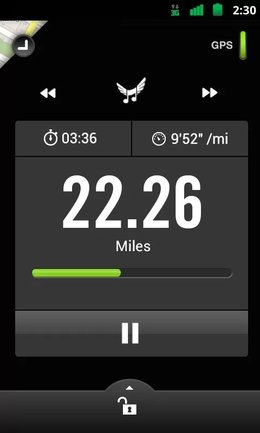
\includegraphics[height=8cm]{images/nr1}
\hspace{0.4in}
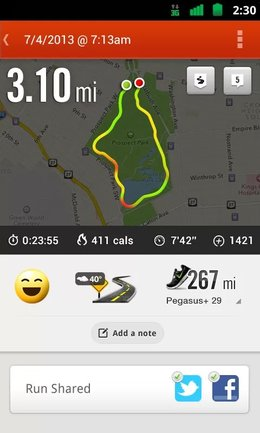
\includegraphics[height=8cm]{images/nr2}
\hspace{0.4in}
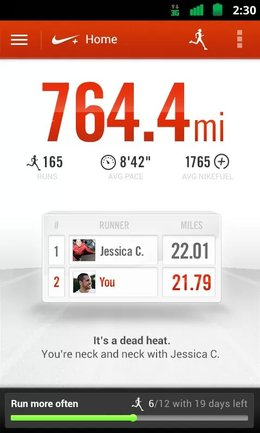
\includegraphics[height=8cm]{images/nr3}
\caption{Στιγμιότυπα χρήσης της εφαρμογής \lt Nike+ Running \gt}
\end{figure}Έχει ως σκοπό να δώσει κίνητρο στον χρήστη για φυσική δραστηριότητα και για αυτό το λόγο του επιτρέπει να προσθέτει φίλους του  να παρακολουθεί την δραστηριότητα τους και να μοιράζεται μαζί τους τις διαδρομές που έχει κάνει, ενώ διαθέτει επιλογή ενώ ο χρήστης κινείται να ακούει τα αγαπημένα του τραγούδια. 

\subsection*{\lt RunKeeper \gt }
Η εφαρμογή \lt Runkeeper \gt της \lt FitnessKeeper \gt έχει ως στόχο να κάνει ευχάριστη την φυσική δραστηριότητα του χρήστη. Λειτουργεί σε κινητά \lt Android \gt και χρησιμοποιεί το \lt GPS \gt της συσκευής για να καταγράψει τρέξιμο, περπάτημα, ποδηλασία και άλλες δραστηριότητες και εμφανίζει στατιστικά για τον ρυθμό, την απόσταση, τον χρόνο, τις θερμίδες που καίει και τον καρδιακό του ρυθμό. Ο χρήστης μπορεί να ενημερώνεται για τα στατιστικά και την πρόοδο του μέσω των ακουστικών του ενώ ταυτόχρονα ακούει συμβουλές προπόνησης. Επίσης, έχει τη δυνατότητα να ακούει μουσική κατά τη διάρκεια της άσκησης και να τραβάει φωτογραφίες για να τις μοιράζεται. Ακόμα, εφαρμογή κρατάει ιστορικό των δραστηριοτήτων και ενημερώνει τον χρήστη όταν φτάσει σε νέο ρεκόρ επίδοσης, ενώ του προτείνει πλάνα άσκησης για να φτάσει σε συγκεκριμένη φυσική κατάσταση.
\begin{figure}[H]
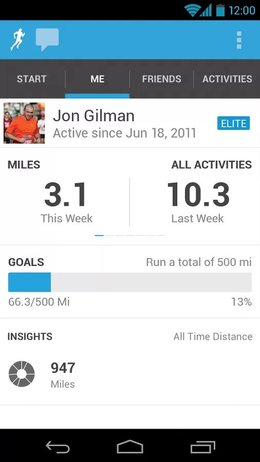
\includegraphics[height=8cm]{images/rk1}
\hspace{0.4in}
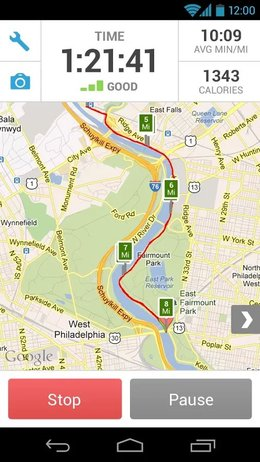
\includegraphics[height=8cm]{images/rk2}
\hspace{0.4in}
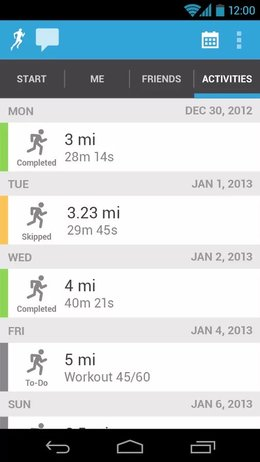
\includegraphics[height=8cm]{images/rk3}
\caption{Στιγμιότυπα χρήσης της εφαρμογής \lt RunKeeper \gt}
\end{figure}
%%%%%%%%%%%%%%%%%%%%%%%%%%%%%%%%%%%%%%%%%%%%%%%%%%%%%%%%%%%%%%%%%%%%%%%%%%%%%%%%%
\section[Δεδομένα Κίνησης και Χαρακτηριστικά]{Δεδομένα Κίνησης και Χαρακτηριστικά}
Στις μέρες μας, οι καθημερινές δραστηριότητες των ανθρώπων δημιουργούν συνεχώς ψηφιακά ίχνη μέσω των ασύρματων δικτύων των κινητών τηλεφώνων. Οι τεχνολογίες προσδιορισμού θέσης όπως το \lt GPS, \gt το \lt UMTS \gt και το \lt GSM, \gt συνεχώς βελτιώνονται ως προς την ακρίβεια της θέσης του χρήστη. Αυτό έχει ως αποτέλεσμα, οι ανθρώπινες δραστηριότητες μπορούν να αναγνωριστούν χρησιμοποιώντας τα δεδομένα κίνησης που καταγράφονται μέσω των κινητών τηλεφώνων. Όμως, με ποιο τρόπο μπορεί να καταγραφεί η κίνηση του χρήστη και τι είδους δεδομένα απαιτούνται για τον καλύτερο προσδιορισμό της κίνησης?

\subsection{Βασικές Αρχές Δεδομένων Κίνησης}

Μια από τις πρώτες προοπτικές ανάλυσης των προτύπων ανθρώπινης δραστηριότητας και της κίνησης στον χωροχρόνο είναι η χρονο-γεωγραφία \lt (time geography). \gt Αναπτύχθηκε από μια ομάδα Σουηδών γεωγράφων το 1970, με σημαντικότερο εκπρόσωπο τον \lt Torsten Hägerstrand. \gt Η χρονο-γεωγραφία έχει χρησιμοποιηθεί από γενιές κοινωνικών επιστημόνων, ιδιαίτερα γεωγράφων και ερευνητών μεταφορών, για την περιγραφή και την ανάλυση των ανθρώπινων δραστηριοτήτων στο χώρο-χρόνο. Θεωρεί και απεικονίζει τις δραστηριότητες ενός ατόμου σε ένα 24-ωρο ως μία συνεχή χρονική ακολουθία στο γεωγραφικό χώρο.Ο αριθμός και οι τοποθεσίες των καθημερινών δραστηριοτήτων ενός ατόμου περιορίζονται από τον διαθέσιμο χρόνο και από ποικίλες υποχρεωτικές δραστηριότητες (π.χ. εργασία).  Η τροχιά της κίνησης  του χρήστη θεωρείται μια διαδρομή στον χωρόχρονο και αναπαρίσταται στον τρισδιάστατο χώρο χρησιμοποιώντας τον οριζόντιο άξονα για την αναπαράσταση του γεωγραφικού χώρου και τον κάθετο άξονα για τον χρόνο. Η αναπαράσταση αυτή ονομάζεται κύβος χωροχρόνου \lt (space-time cube) \gt και απεικονίζεται στο Σχήμα \ref{fig:space-timeCube} \cite{giannotti2008mobility}\cite{geovisualization}

\begin{figure}[H]
\centering
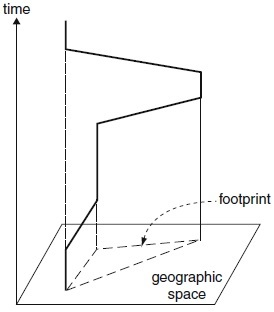
\includegraphics{images/space_time_cube}
\caption{Απεικόνιση του \lt space-time cube\gt \cite{giannotti2008mobility}}
\label{fig:space-timeCube}
\end{figure}

Η γραμμή αναπαριστά τις κινήσεις μιας οντότητας, για παράδειγμα, ας θεωρήσουμε έναν εργαζόμενο, ο οποίος αρχικά ήταν στο σπίτι, μετά πήγε στη δουλειά του και έμεινε εκεί για ένα χρονικό διάστημα, μετά πήγε στο σουπερμάρκετ για ψώνια και αφού έμεινε κι εκεί για λίγο, γύρισε σπίτι. Οι κάθετες γραμμές ερμηνεύονται σαν την παραμονή του χρήστη σε συγκεκριμένο μέρος (σπίτι, εργασία, σουπερμάρκετ). Τα κεκλιμένα τμήματα της γραμμής υποδεικνύουν κινήσεις. Όσο πιο αργή είναι η κίνηση, τόσο πιο απότομη είναι η γραμμή. Η ευθεία γραμμή δείχνει ότι το άτομο κινείται με σταθερή ταχύτητα, η οποία είναι συνήθως μια προσέγγιση της  πραγματικής συμπεριφοράς. Η απεικόνιση αυτής της αναπαράστασης σε χάρτη είναι το αποτύπωμα της διαδρομής που ακολούθησε ο χρήστης. 

\subsection{Χαρακτηριστικά Κίνησης}
Για την αναγνώριση της δραστηριότητας του χρήστη πρέπει να εξεταστούν πολλοί παράγοντες της κίνησης. Αρχικά, τα χαρακτηριστικά της κάθε κίνησης όπως για παράδειγμα η ταχύτητα και η κατεύθυνση, η τροχιά της κίνησης που ακολουθεί ο χρήστης αλλά και τα χαρακτηριστικά του χρήστη. Παράλληλα, πολλά συμπεράσματα μπορούν να εξαχθούν για την φύση της κίνησης παρατηρώντας το περιβάλλον της και τα συμβάντα που εξελίσσονται σε αυτό. \cite{giannotti2008mobility}

Η έννοια της \emph{κίνησης} μπορεί να οριστεί σαν την μεταβολή της φυσικής θέσης μιας οντότητας σε σχέση με ένα σύστημα αναφοράς στο οποίο μπορεί να προσδιοριστεί η θέση της οντότητας. Το σύστημα αναφοράς συνήθως είναι ένας γεωγραφικός χώρος.

Η κίνηση μιας οντότητας αποτελείται από \emph{τροχιές}, δηλαδή από τις διαδρομές που ακολουθεί η οντότητα στον χώρο κατά την κίνηση της. Μια διαδρομή δεν δημιουργείται ποτέ στιγμιαία, αντίθετα απαιτεί ένα χρονικό διάστημα. Για αυτό τον λόγο, η τροχιά στην οποία κινείται μια οντότητα πρέπει να συνδέεται με τον χρόνο και μπορεί να περιγραφεί από μια σειρά εγγραφών της μορφής (χρονική στιγμή, θέση). Ο τρόπος καταγραφής μιας τροχιάς ποικίλει, καθώς διαφέρει ανάλογα με τον τρόπο παρατήρησης της κίνησης. 

\subsubsection*{Τρόποι καταγραφής κίνησης}
\begin{itemize}
  \item \emph{Χρονική.} Η καταγραφή της θέσης της οντότητας γίνεται ανά τακτά χρονικά διαστήματα (π.χ. ανά λεπτό).
  \item \emph{Με βάση την μεταβολή θέσης.} Γίνεται καταγραφή όταν η θέση της οντότητας διαφέρει από την προηγούμενη.
  \item	\emph{Με βάση τη θέση κοντά σε συγκεκριμένη τοποθεσία.} Καταγραφή της θέσης όταν η οντότητα πλησιάζει σε μια συγκεκριμένη τοποθεσία.
  \item \emph{Με βάση κάποιο συμβάν.} Η θέση της οντότητας καταγράφεται όταν συμβεί κάποιο συγκεκριμένο γεγονός, συνήθως αφορά δραστηριότητες των ίδιων οντοτήτων.  
\end{itemize}

Όσον αφορά στα χαρακτηριστικά της κίνησης που μελετούνται, μπορούν να διακριθούν σε δυο κατηγορίες ανάλογα με το αν αναφέρονται σε χρονική στιγμή ή σε χρονικό διάστημα.
\subsubsection*{Χαρακτηριστικά χρονικής στιγμής της κίνησης}
\begin{itemize}
  \item \lt Timestamp \gt της συγκεκριμένης χρονικής στιγμής
  \item Θέση της οντότητας στον χώρο
  \item	Κατεύθυνση
  \item Ταχύτητα
  \item Αλλαγή κατεύθυνσης
  \item Επιτάχυνση (αλλαγή ταχύτητας)
  \item Συνολικός χρόνος κίνησης
  \item Συνολική απόσταση που έχει διανυθεί
\end{itemize}

\subsubsection*{Χαρακτηριστικά χρονικού διαστήματος της κίνησης}
\begin{itemize}
  \item Γεωμετρικό σχήμα της κίνησης στον χώρο
  \item Απόσταση που έχει διανυθεί στον χώρο
  \item	Χρονική διάρκεια της κίνησης
  \item Διάνυσμα της κίνησης (από την αρχική στην τελική θέση)
  \item Μέση και μέγιστη τιμή της ταχύτητας
  \item Δυναμική συμπεριφορά της ταχύτητας (σταθερή ταχύτητα, επιτάχυνση, επιβράδυνση, μηδενική ταχύτητα)
  \item Δυναμική συμπεριφορά της κατεύθυνσης (ευθεία, καμπυλόγραμμη, κυκλική κίνηση)
\end{itemize}

\subsubsection*{Χώρος}
Ως χώρος μπορεί να θεωρηθεί το σύνολο από τοποθεσίες και μέρη, με την ιδιότητα να μπορεί να οριστεί η απόσταση μεταξύ τους. Για τη διάκριση των διαφορετικών τοποθεσιών στον χώρο πρέπει να θεωρηθεί ένα σύστημα αναφοράς, όπως ένα σύστημα συντεταγμένων. Ανάλογα με τις απαιτήσεις του προβλήματος, ο χώρος μπορεί να θεωρηθεί ως δισδιάστατος ή τρισδιάστατος, δηλαδή ένα σημείο μπορεί να περιγραφεί από δύο ή τρεις συντεταγμένες αντίστοιχα.

Ο φυσικός χώρος είναι συνεχής, το οποίο σημαίνει ότι αποτελείται από άπειρο αριθμό από τοποθεσίες. Από την άλλη πλευρά, κάποιες φορές μπορεί να είναι χρήσιμο να θεωρούμε τον χώρο διακριτό ή από πεπερασμένο αριθμό από τοποθεσίες. Σε κάποιες περιπτώσεις, η διακριτοποίηση του χώρου μπορεί να είναι απαραίτητη, όταν οι θέσεις των οντοτήτων δεν μπορούν να προσδιοριστούν με ακρίβεια αλλά με την έννοια ευρύτερης περιοχής όπως για παράδειγμα περιοχές δικτύου κινητής τηλεφωνίας, περιοχές μιας πόλης ή χώρες.

Ο χώρος μπορεί να δομηθεί με διάφορους τρόπους για να επιτευχθεί καλύτερη καταγραφή της κίνησης μιας οντότητας. Ένας τρόπος είναι η ιεραρχική διαίρεση, για παράδειγμα μια χώρα χωρίζεται σε επαρχίες, οι επαρχίες σε δήμους και οι κοινότητες σε επαρχίες. Περιοχές μπορούν να προκύψουν ακόμα από  γεωγραφική διαίρεση, δηλαδή δημιουργώντας κελιά στον χώρο με συγκεκριμένο μέγεθος (π.χ. 1 \lt km2 \gt). Επίσης, ένας πολύ κοινός τρόπος δόμησης του φυσικού χώρου είναι με βάση το οδικό δίκτυο.

Γενικά, οι πιθανοί τρόποι με τους οποίους μπορεί να προσδιοριστεί η θέση μιας οντότητας στον γεωγραφικό χώρο περιγράφονται παρακάτω.
\begin{itemize}
\item\emph{Αναφορά με βάση συντεταγμένες}. Οι θέσεις ορίζονται με αριθμούς που αντιστοιχούν στη γραμμική ή γωνιακή απόσταση από καθορισμένους άξονες ή γωνίες.
\item\emph{Αναφορά με βάση τη διαίρεση του χώρου}. Αναφέρεται σε περιοχές μιας γεωμετρική ή σημασιολογική διαίρεση του χώρου, ενδεχομένως ιεραρχική.
\item\emph{Γραμμική αναφορά}.  Αναφέρονται σε σχετικές θέσεις κατά μήκος γραμμικών αντικειμένων όπως δρόμοι, ποτάμια, αγωγοί.  Για παράδειγμα, ονόματα δρόμων καθώς και αριθμούς σπιτιών ή κωδικούς δρόμων και αποστάσεις από κάποιο από τα άκρα.
\end{itemize}


\subsubsection*{Χρόνος}
Από μαθηματική άποψη, ο χρόνος είναι μια συνεχής σειρά στοιχείων με γραμμική διάταξη και αποστάσεις μεταξύ των στοιχείων, όπου τα στοιχεία είναι στιγμές ή θέσεις στο χρόνο. Όπως συμβαίνει και με τον χώρο, απαιτείται ένα σύστημα αναφοράς για τον προσδιορισμό των χρονικών στιγμών στα δεδομένα. Στις περισσότερες περιπτώσεις, ως σύστημα αναφοράς χρησιμοποιείται το Γρηγοριανό ημερολόγιο \lt (Gregorian calendar), \gt και η διαίρεση του χρόνου σε ημέρες, μήνες, ώρες, λεπτά και δευτερόλεπτα. Η ώρα της ημέρας μπορεί να προσδιοριστεί με τη ζώνη ώρας της περιοχής στην οποία καταγράφονται τα δεδομένα ή με βάση την ζώνη ώρας του \lt Greenwich (GMT). \gt Υπάρχουν βέβαια περιπτώσεις, στις οποίες τα δεδομένα αναφέρονται σε σχετικές χρονικές στιγμές, για παράδειγμα  ο χρόνος που έχει παρέλθει από την έναρξη μιας διαδικασίας ή της παρατήρησης.

Ο πραγματικός χρόνος περιλαμβάνει επίσης χρονικούς κύκλους που προκύπτουν από την καθημερινή και την ετήσια περιστροφή της γης. Αυτοί οι φυσικοί χρονικοί κύκλοι γίνονται αντιληπτοί με τη φυσική ροή του χρόνου, για παράδειγμα οι ημερομηνίες επαναλαμβάνονται κάθε χρόνο και οι ώρες κάθε μέρα. Εκτός από τους φυσικούς χρονικούς κύκλους, υπάρχουν και αυτοί που σχετίζονται με τις δραστηριότητες των ανθρώπων, για παράδειγμα μια δραστηριότητα μπορεί να γίνεται μια φορά τη μέρα ή τη βδομάδα. Για τη ανάλυση των κινήσεων, είναι πολύ σημαντικό να είναι γνωστοί οι χρονικοί κύκλοι που σχετίζονται με την κίνηση. Οι ιδιότητες κάθε χρονικού κύκλου μπορεί να διαφέρουν και αυτές οι διαφορές μπορεί να έχουν σημαντική επίδραση στις κινήσεις. Για παράδειγμα, οι κινήσεις των ανθρώπων τις καθημερινές διαφέρουν από τα Σαββατοκύριακα. 

Όμως, η ετερογένεια των ιδιοτήτων κάθε χρονικής στιγμής δεν μπορεί να εκφραστεί σαφώς στα δεδομένα και για αυτό τον λόγο δεν είναι δυνατό να ληφθούν υπόψη αυτόματα στην ανάλυση των δεδομένων. Η ανάλυση των ιδιοτήτων του χώρου εξαρτάται σημαντικά από την ικανότητα του αναλυτή να χρησιμοποιήσει τις γνώσεις του και είναι απαραίτητο οι μέθοδοι και τα εργαλεία που θα χρησιμοποιήσει για την ανάλυση τους να του δίνουν αυτή τη δυνατότητα. 

\subsubsection*{Κινούμενες οντότητες και τα χαρακτηριστικά τους}
Εκτός από τα χαρακτηριστικά της κίνησης που αναφέρθηκαν, οι οντότητες που κινούνται έχουν τα δικά τους χαρακτηριστικά, τα οποία επηρεάζουν την κίνηση τους και πρέπει να ληφθούν υπόψη κατά την ανάλυση των δεδομένων κίνησης. Έτσι, οι κινήσεις των ανθρώπων μπορεί να επηρεάζονται σημαντικά από το επάγγελμα, την ηλικία, την κατάσταση υγείας, την οικογενειακή κατάσταση και από άλλα χαρακτηριστικά. Ακόμα, μπορεί να αναλυθεί ο σκοπός της κίνησης ενός ανθρώπου, καθώς μπορεί έτσι να καθοριστεί η διαδρομή που θα ακολουθήσει και η ταχύτητα κίνησης του. Τα χαρακτηριστικά της κίνησης μπορεί επίσης να εξαρτώνται από τις δραστηριότητες των ανθρώπων ενώ κινούνται. Για παράδειγμα, η κίνηση ενός ανθρώπου σε ένα κατάστημα, διαφέρει από την κίνηση στον δρόμο. Επίσης, τα χαρακτηριστικά της κίνησης είναι διαφορετικά όταν ένας άνθρωπος απλά περπατάει από όταν περπατάει και μιλάει στο τηλέφωνο ταυτόχρονα.

\subsubsection*{Σχετικά φαινόμενα και συμβάντα}
Οι κινήσεις που εμφανίζονται σε ένα περιβάλλον, επηρεάζονται από τα διάφορα συμβάντα αυτού του περιβάλλοντος. Οι κινήσεις των ανθρώπων επηρεάζονται από το κλίμα και τις καιρικές συνθήκες, από τις αθλητικές και πολιτιστικές εκδηλώσεις, από τις τρέχουσες νομοθετικές ρυθμίσεις, από τα τέλη διοδίων και τις τιμές των καυσίμων, από τα τροχαία ατυχήματα και ούτω καθεξής. Για την ανίχνευση τέτοιων επιρροών κατά την ανάλυση των δεδομένων, ο αναλυτής πρέπει να χρησιμοποιήσει πρόσθετα στοιχεία και γνώσεις.
%%%%%%%%%%%%%%%%%%%%%%%%%%%%%%%%%%%%%%%%%%%%%%%%%%%%%%%%%%%%%%%%%%%%%%%%%%%%%%%%%
\section[Τεχνικές Αναγνώρισης Κίνησης]{Τεχνικές Αναγνώρισης Κίνησης}
Η αναγνώριση της ανθρώπινης δραστηριότητας έχει συγκεντρώσει μεγάλο ενδιαφέρον και έχουν πραγματοποιηθεί πολλές έρευνες για τον εντοπισμό πληροφοριών, χρήσιμων για την αναγνώριση κίνησης. Η αναγνώριση κίνησης μπορεί εύκολα να υλοποιηθεί σε κινητά τηλέφωνα χρησιμοποιώντας τους ενσωματωμένους αισθητήρες της συσκευής και γι’ αυτό τον λόγο έχουν αναπτυχθεί πολλές εφαρμογές για \lt smartphone. \gt Οι κυριότερες τεχνικές εξόρυξης δεδομένων που χρησιμοποιούν οι υπάρχουσες εφαρμογές για την αναγνώριση της ανθρώπινης δραστηριότητας αναλύονται παρακάτω.
\subsection[Κατηγοριοποίηση]{Κατηγοριοποίηση (\lt Classification) \gt}
Οι περισσότεροι ερευνητές που χρησιμοποιούν την τεχνική της κατηγοριοποίησης για να ανιχνεύσουν την δραστηριότητα του χρήστη, καταγράφουν χαρακτηριστικά \lt (attributes) \gt της κίνησης τα οποία μπορούν να διακριθούν σε τρεις βασικές κατηγορίες. Παρακάτω περιγράφονται τα χαρακτηριστικά που ανήκουν σε κάθε κατηγορία.
\begin{itemize}
\item\emph{Μεγέθους}. Αυτή η κατηγορία αναφέρεται σε χαρακτηριστικά που βασίζονται σε τιμές που καταγράφουν οι αισθητήρες της συσκευής. Συνήθως οι τιμές είναι συντεταγμένες, μέση τιμή, τυπική απόκλιση, ελάχιστη και μέγιστη τιμή, μέση απόλυτη διαφορά και άλλες. 
\item\emph{Συχνότητας}. Είναι τα χαρακτηριστικά που βασίζονται στις τιμές συχνότητας των αισθητήρων. Το πιο συνηθισμένο μέγεθος είναι από τον μετασχηματισμό Fourier (FFT). Άλλα χαρακτηριστικά αυτής της κατηγορίας είναι η εντροπία της συχνότητας, η μέγιστη συχνότητα, η μέση τιμή, η τυπική απόκλιση και η ενέργεια του μετασχηματισμού Fourier.
\item\emph{Συσχέτισης}. Πολλοί ερευνητές χρησιμοποιούν ως χαρακτηριστικά, τις συσχετίσεις μεταξύ των υπολοίπων χαρακτηριστικών.
\end{itemize}
	Όσον αφορά στον αλγόριθμο κατηγοριοποίησης που μπορούμε να χρησιμοποιήσουμε για να κατηγοριοποιήσουμε διαφορετικές δραστηριότητες του χρήστη, η επιλογή του εξαρτάται από την επεξεργαστική ισχύ του συστήματος που θα εκτελεστεί ο αλγόριθμος. Δηλαδή αν ο αλγόριθμος εκτελεστεί σε \lt server \gt είναι προφανές ότι η επεξεργαστική ισχύς του μηχανήματος θα είναι αρκετά πιο μεγάλη από την επεξεργαστική ισχύ ενός \lt smartphone. \gt Οι περισσότεροι ερευνητές χρησιμοποιούν αλγόριθμους κατηγοριοποίησης με επίβλεψη. Αυτοί οι αλγόριθμοι εκπαιδεύονται με κατηγοριοποιημένα δείγματα για τη δημιουργία μοντέλου κατηγοριοποίησης, το οποίο στη συνέχεια θα χρησιμοποιηθεί για την κατηγοριοποίηση των δεδομένων εισόδου. Οι πιο συνηθισμένοι αλγόριθμοι που χρησιμοποιούνται για αναγνώριση κίνησης είναι τα Δέντρα απόφασης \lt (Decision Trees), \gt ο κ – κοντινότερος γείτονας \lt (kNN), \gt ο \lt Naïve Bayes, \gt ο \lt SVM \gt και τα Νευρωνικά δίκτυα. Όμως, η κατηγοριοποίηση με επίβλεψη χρειάζεται μεγάλη επεξεργαστική ισχύ για να δημιουργήσει μοντέλο από δεδομένα εκπαίδευσης και για αυτόν τον λόγο οι περισσότερες υλοποιήσεις έχουν γίνει σε \lt servers. \gt Βέβαια κάποιοι άλλοι ερευνητές, δημιουργούν το μοντέλο κατηγοριοποίησης εκτελώντας τον αλγόριθμο σε ένα μηχάνημα και έπειτα μεταφέρουν το μοντέλο στο τηλέφωνο για την κατηγοριοποίηση των δεδομένων εισόδου. Ακόμα, η αξιολόγηση των αλγορίθμων κατηγοριοποίησης είναι πολύ σημαντική, καθώς δείχνει ποιος αλγόριθμος αποδίδει καλύτερα. Οι δημοφιλέστερες μέθοδοι αξιολόγησης που χρησιμοποιούνται είναι οι \lt n-fold cross validation (\gt συνήθως \lt 10-fold) \gt και τα μέτρα \lt precision, recall, F-measure \gt και \lt accuracy. \gt \cite{bin2012classification}

\subsection[Συσταδοποίηση τροχιών κίνησης]{Συσταδοποίηση τροχιών κίνησης (\lt Spatemporal/Trajectory Clustering) \gt}
Η συσταδοποίηση των τροχιών των κινούμενων αντικειμένων, παρουσιάζει μεγάλο ενδιαφέρον στην ερευνητική κοινότητα και για αυτόν τον λόγο υπάρχει μεγάλος αριθμός ερευνών που εξετάζουν διαφορετικές τεχνικές συσταδοποίησης με σκοπό τη βελτίωση των αποτελεσμάτων τους. Η τροχιά (trajectory) κίνησης ενός χρήστη, αναφέρεται σε μια χρονική ακολουθία  τοποθεσιών με τη σειρά που ο χρήστης τις επισκέφτηκε \cite{Giannotti:2010}. Η συσταδοποίηση των τροχιών έχει ως στόχο την ομαδοποίηση των τροχιών σε συστάδες όμοιων τροχιών\cite{marketos2009mobility}. Οι τροχιές των κινούμενων οντοτήτων πολύ συχνά περιέχουν επαναλαμβανόμενα μοτίβα κίνησης από τα οποία με την τεχνική της συσταδοποίησης είναι δυνατόν να ανιχνευτούν όμοια μοτίβα με σκοπό την αναγνώριση της δραστηριότητας\cite{SungFR12}. 

Οι μέθοδοι που υπάρχουν μέχρι σήμερα στη βιβλιογραφία ακολουθούν δυο βασικές προσεγγίσεις. Η πρώτη προσέγγιση έχει ως στόχο να βρει ένα μέτρο ομοιότητας μεταξύ των τροχιών. Ορίζοντας την απόσταση μεταξύ αντικειμένων καθορίζεται ποιες τροχιές πρέπει να βρίσκονται στην ίδια συστάδα και στη συνέχεια ποιες είναι οι συστάδες που πρέπει να ανιχνευτούν. Ένας βασικός τρόπος για οριστεί η απόσταση είναι να εξεταστούν τροχιές χρηστών που είναι παρόμοιες, για παράδειγμα τροχιές στις οποίες κάθε χρονική στιγμή οι χρήστες βρίσκονται σχεδόν στην ίδια τοποθεσία. Μια απλή προσέγγιση για τη μοντελοποίηση αυτής της σύγκρισης είναι να θεωρηθούν οι τροχιές διανύσματα των συντεταγμένων και να γίνει σύγκριση των διανυσμάτων χρησιμοποιώντας ένα μέτρο απόστασης, όπως η Ευκλείδεια απόσταση.\cite{giannotti2008mobility}

Η δεύτερη μέθοδος συσταδοποίησης των τροχιών κίνησης, δεν κάνει χρήση μέτρων ομοιότητας αλλά αντιμετωπίζει κάθε τροχιά ως ένα αντικείμενο και αναζητά ομάδες τροχιών που κινούνται μαζί\cite{giannotti2008mobility}. Μια αποτελεσματική προσέγγιση χρησιμοποιούν οι \lt Lee \gt και συν. \cite{Lee:2007}, με τον αλγόριθμο \lt TRACLUS. \gt Αρχικά χωρίζουν τις τροχιές σε μια σειρά υποσυνόλων κάνοντας χρήση του \lt MDL (Minimum Description Length) \gt και έπειτα δημιουργούν συστάδες όμοιων υποσυνόλων λαμβάνοντας υπόψη την πυκνότητα τους. Για κάθε συστάδα, η τροχιά που περιγράφει την συνολική κίνηση των υποσυνόλων που ανήκουν στην ίδια συστάδα, είναι η τροχιά που αντιπροσωπεύει τη συστάδα. Αντίθετα, οι \lt Giannotti \gt και συν. \cite{Giannotti:2010} προτείνουν την έννοια των μοτίβων κίνησης και παρουσιάζουν έναν αλγόριθμο για την ανίχνευση τους στις τροχιές. Τα μοτίβα κίνησης αντιπροσωπεύουν σύνολα τοποθεσιών ενδιαφέροντος που σχετίζονται χρονικά, και μπορούν να είναι προκαθορισμένα από τον χρήστη ή να ανακαλυφθούν με κάποιο αλγόριθμο συσταδοποίησης βασισμένο στην πυκνότητα των συστάδων. Ταυτόχρονα, οι \lt Sung,  Feldman \gt και \lt Rus\gt \cite{SungFR12}, παρουσιάζουν έναν αλγόριθμο για την εξαγωγή μοτίβων κίνησης από τις τροχιές και χρησιμοποιούν τα αποτελέσματα για να δημιουργήσουν ένα Μαρκοβιανό μοντέλο το οποίο θα κάνει πρόβλεψη της κίνησης για την κάθε οντότητα.

\subsection[\lt Conditional Random Fields (CRF) \gt]{\lt Conditional Random Fields (CRF)\gt}
Μια διαφορετική προσέγγιση για την αναγνώριση δραστηριότητας παρουσιάζουν οι \lt Liao, Lin \gt και \lt Fox \gt κάνοντας χρήση ιεραρχικών μοντέλων \lt CRF \gt σε δεδομένα \lt GPS \gt για την εξαγωγή σημαντικών τοποθεσιών και δραστηριοτήτων του χρήστη. 

Αρχικά, χωρίζουν τα δεδομένα \lt GPS \gt ομαδοποιώντας τα με βάση τη σχέση τους στον χώρο και κάθε \lt GPS \gt στίγμα το αντιστοιχούν στον πιο κοντινό δρόμο. Για να δημιουργήσουν μια σωστή συσχέτιση μεταξύ των τοποθεσιών, δημιουργούν ένα μοντέλο \lt CRF \gt με βάση τη χωρική σχέση μεταξύ τους.

Αφού χωρίσουν τις τοποθεσίες, ο αλγόριθμος τους κάνει εκτίμηση για την δραστηριότητα που εκτελείται σε κάθε σύνολο και ξεχωρίζει τις σημαντικές τοποθεσίες κάθε χρήστη. Για να επιτευχθεί αυτό, δημιουργεί ένα νέο μοντέλο \lt CRF \gt το οποίο περιέχει έναν κρυμμένο κόμβο που αντιστοιχεί στη δραστηριότητα σε κάθε σύνολο που δημιουργήθηκε από τις καταγεγραμμένες \lt GPS \gt συντεταγμένες. Κάθε κόμβος δραστηριότητας είναι συνδεδεμένος με μερικά χαρακτηριστικά που προκύπτουν από τις πληροφορίες που προέρχονται από τη διαίρεση των δεδομένων, όπως ημερομηνία και ώρα, μέση ταχύτητα, πληροφορίες για τα σημεία ενδιαφέροντος που βρίσκονται κοντά. Έπειτα, στο μοντέλο \lt CRF \gt που δημιουργήθηκε, εφαρμόζει τον αλγόριθμο \lt Naïve Bayes \gt για να ανιχνεύσει την δραστηριότητα του χρήστη σε κάθε τοποθεσία. 

Στη συνέχεια, χρησιμοποιεί τις ακολουθίες στις οποίες ο χρήστης πραγματοποιεί τον ίδιο τύπο κίνησης για να αναζητήσει τις σημαντικές τοποθεσίες του χρήστη. Αυτό γίνεται κατηγοριοποιώντας ξεχωριστές δραστηριότητες στην ίδια ακολουθία, με βάση το αν ανήκουν σε μια συγκεκριμένη τοποθεσία και θεωρώντας ότι όλες οι εγγραφές στις οποίες παρατηρείται μια συγκεκριμένη δραστηριότητα αποτελούν μια σημαντική τοποθεσία. 

Η προσέγγιση τους παρουσιάζει ενδιαφέρον, καθώς ο αλγόριθμος που χρησιμοποιούν έχει αρκετά μεγάλο ποσοστό ακρίβειας (86\%), ενώ η ταυτόχρονη εκτίμηση δραστηριότητας και τοποθεσίας αυξάνει την ποιότητα του αποτελέσματος. Αυτό συμβαίνει γιατί η κάθε θέση συνδέει τις δραστηριότητες που συμβαίνουν στην χωρική περιοχή της και οι δραστηριότητες αναγνωρίζονται με πιο συνεπή τρόπο.\cite{Liao:2007}

%%%%%%%%%%%%%%%%%%%%%%%%%%%%%%%%%%%%%%%%%%%%%%%%%%%%%%%%%%%%%%%%%%%%%%%%%%%%%%%%%
%%%%%%%%%%%%%%%%%%%%%%%%%%%%%%%%%%%%%%%%%%%%%%%%%%%%%%%%%%%%%%%%%%%%%%%%%%%%%%%%%
\chapter[Σχεδιασμός]{Σχεδιασμός}
\label{Chapter5}
\section[Το περιβάλλον \lt Eclipse\gt]{Το περιβάλλον \lt Eclipse\gt}
Το \lt Eclipse IDE \gtείναι ένα περιβάλλον ανάπτυξης λογισμικού, το οποίο αρχικά αναπτύχθηκε από την \lt IBM \gtως εργαλείο ανάπτυξης \lt Java \gtμε σκοπό να αντικαταστήσει το ήδη υπάρχον περιβάλλον \lt Visual Age, \gtαλλά κυκλοφόρησε ως λογισμικό ανοιχτού κώδικα τον Νοέμβριο του 2001\cite{Burnette:2005}. To 2004, ο μη κερδοσκοπικός οργανισμός \lt Eclipse Foundation \gtκαι το επιστημονικό του προσωπικό ανέλαβε ολοκληρωτικά τον έλεγχο της πλατφόρμας \lt Eclipse. \gtΤο \lt Eclipse \gtσήμερα αποτελεί το πιο διαδεδομένο περιβάλλον ανάπτυξης για \lt Java,  \gtενώ ταυτόχρονα εξαιτίας της επεκτάσιμης αρχιτεκτονικής του χρησιμοποιείται ως εργαλείο ανάπτυξης για πολλές άλλες γλώσσες προγραμματισμού\cite{Cinar:2012}.

Η πλατφόρμα \lt Eclipse \gtσχεδιάστηκε με στόχο την ανάπτυξη ολοκληρωμένων περιβαλλόντων ανάπτυξης. Αποτελεί ένα εύκολα επεκτάσιμο περιβάλλον, παρέχοντας μηχανισμούς που επιτρέπουν την εγκατάσταση επιπρόσθετων εργαλείων τα οποία μπορούν να κάνουν χρήση άλλων διεπαφών ανάπτυξης εφαρμογών \lt (APIs). \gtΗ αρχιτεκτονική της πλατφόρμας \lt Eclipse \gtείναι δομημένη με τέτοιο τρόπο ώστε να επιτρέπει την χρήση πρόσθετων εργαλείων, όπως φαίνεται στο Σχήμα \ref{fig:eclipseSDK}\cite{Cinar:2012}. 
\begin{figure}[H]
\centering
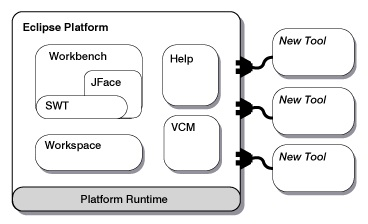
\includegraphics{images/eclipseSDK}
\caption{Η αρχιτεκτονική της πλατφόρμας \lt Eclipse\gt}
\label{fig:eclipseSDK}
\end{figure}

Τα πρόσθετα εργαλεία αποτελούν την μικρότερη μονάδα της πλατφόρμας \lt Eclipse, \gtτα οποία είναι δομημένα κομμάτια κώδικα που προσφέρουν επιπλέον λειτουργικότητα στην πλατφόρμα. Για την ανάπτυξη μιας εφαρμογής για \lt Android, \gtχρησιμοποιείται ένα σύνολο πρόσθετων που είναι γνωστό ως \lt Android Development Toolkit (ADT) \gtτο οποίο επεκτείνει τα υπάρχουσα εργαλεία της \lt Java (JDK) \gtγια  να προσφέρει συγκεκριμένες λειτουργίες που απαιτούνται για τον προγραμματισμό σε \lt Android.\gt
\section{Το \lt ADT plug-in\gt}
Το \lt ADT (Android Developer Tools) \gtείναι ένα πρόσθετο για το \lt Eclipse \gtτο οποίο περιλαμβάνει ένα σύνολο εργαλείων που ενσωματώνονται στο περιβάλλον του \lt Eclipse. \gtΠροσφέρει πρόσβαση σε πολλές λειτουργίες που διευκολύνουν την ανάπτυξη εφαρμογών \lt Android. \gtΤο \lt ADT \gtπαρέχει γραφικό περιβάλλον για την πρόσβαση στα εργαλεία του \lt SDK \gtκαθώς και ένα εργαλείο σχεδιασμού γραφικού περιβάλλοντος για την εύκολη και γρήγορη δημιουργία της διεπαφής χρήστη της εφαρμογής που αναπτύσσεται.

Η εγκατάσταση του \lt ADT \gtδιευκολύνει τη δημιουργία και την δοκιμή εφαρμογών \lt Android, \gtεπιτρέποντας την δημιουργία, την ανάπτυξη και τον εντοπισμό σφαλμάτων της εφαρμογής ενώ επεκτείνει το \lt documentation \gtτης \lt Java \gtγια τα \lt APIs \gtτου \lt Android. \gtΑκόμα, ενσωματώνει τα εργαλεία του \lt Android SDK, \gtπροσθέτοντας τα αντίστοιχα μενού στο περιβάλλον του \lt Eclipse. \gtΕπιπλέον, το \lt ADT \gtσυμπεριλαμβάνει επεξεργαστή \lt XML \gtαρχείων, το οποίο επιτρέπει την επεξεργασία των \lt XML \gtαρχείων του \lt Android  \gtκαι τη δημιουργία γραφικών διεπαφών χρήστη.
\section{Το εργαλείο \lt Android SDK\gt}
Το \lt Android SDK (Software Development Kit) \gtπεριλαμβάνει ένα σύνολο εργαλείων, τα οποία είναι απαραίτητα για την ανάπτυξη εφαρμογών για συσκευές \lt Android \gtκαι ενσωματώνεται στο περιβάλλον \lt Eclipse \gtμέσω του \lt ADT. \gtΤα εργαλεία διακρίνονται σε δυο κατηγορίες: εργαλεία \lt SDK \gtκαι εργαλεία πλατφόρμας \lt Android. \gtΤα εργαλεία \lt SDK \gtείναι ανεξάρτητα από την έκδοση \lt Android \gtγια την οποία προορίζεται η εφαρμογή, ενώ τα εργαλεία πλατφόρμας προσαρμόζονται ώστε να υποστηρίζουν τα χαρακτηριστικά του κάθε \lt API Level \gtπου χρησιμοποιείται.
\subsection*{Τα εργαλεία \lt SDK\gt}
Η χρήση των εργαλείων \lt SDK \gtείναι απαραίτητη για την ανάπτυξη εφαρμογών \lt Android \gtστο περιβάλλον \lt Eclipse\gt, τα πιο σημαντικά εργαλεία περιγράφονται παρακάτω.
\subsection{\lt SDK Manager\gt}
\begin{figure}[H]
\centering
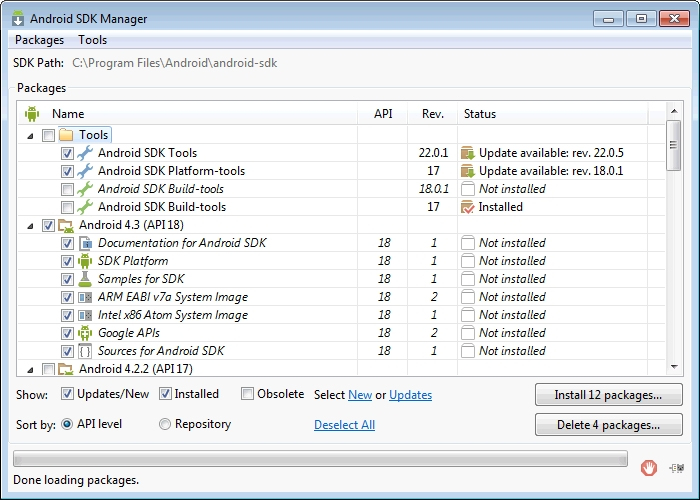
\includegraphics[height=9cm]{images/sdk_manager}
\caption{Στιγμιότυπο του \lt SDK Manager.\gt}
\label{fig:SDKmanager}
\end{figure}
Ο \lt SDK Manager\gt, διαχειρίζεται το \lt Android SDK \gtχωρίζοντας τα εργαλεία και τις πλατφόρμες σε πακέτα και επιτρέπει στον χρήστη να κατεβάσει τα πακέτα που του είναι απαραίτητα. O \lt SDK Manager \gtεμφανίζει τα πακέτα \lt SDK \gtπου είναι διαθέσιμα, όσα έχουν ήδη εγκατασταθεί αλλά και αυτά για τα οποία υπάρχουν διαθέσιμες ενημερώσεις όπως φαίνεται στο Σχήμα \ref{fig:SDKmanager}.
\subsection{Προσομοιωτής κινητής συσκευής \lt (Android Emulator)\gt}
\begin{figure}[H]
\centering
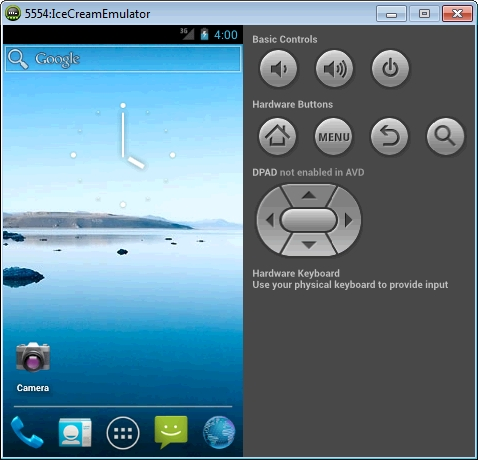
\includegraphics[height=9cm]{images/emulator}
\caption{Στιγμιότυπο του \lt Android Emulator\gt}
\label{fig:emulator}
\end{figure}
Το \lt Android SDK \gtπεριλαμβάνει έναν προσομοιωτή κινητής συσκευής, ο οποίος τρέχει στον υπολογιστή του χρήστη και του επιτρέπει να αναπτύσσει και να δοκιμάζει εφαρμογές \lt Android \gtχωρίς τη χρήση φυσικής συσκευής.
\subsection{\lt AVD Manager\gt}
\begin{figure}[H]
\centering
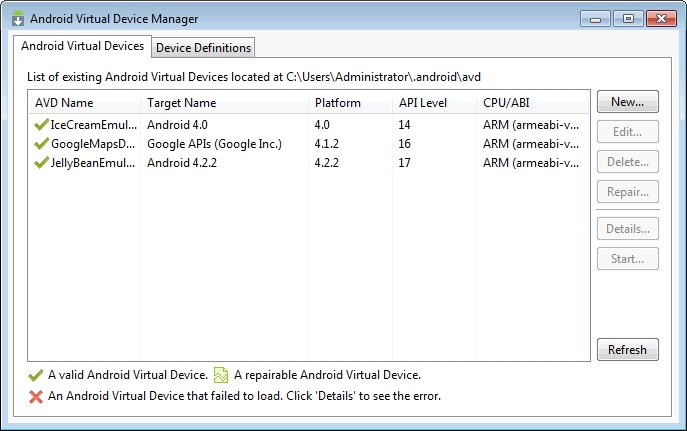
\includegraphics[height=9cm]{images/avd_manager}
\caption{Στιγμιότυπο του \lt AVD Manager.\gt}
\label{fig:AVDmanager}
\end{figure}
Ο \lt AVD (Android Virtual Device) Manager \gtαποτελεί ένα γραφικό περιβάλλον για τη διαχείριση των ρυθμίσεων των εικονικών συσκευών \lt Android\gt. Μια συσκευή 
\lt AVD \gtορίζει τις ρυθμίσεις διαμόρφωσης του προσομοιωτή συσκευής \lt Android \gtεπιτρέποντας την αναπαράσταση διαφορετικών συσκευών που τρέχουν λειτουργικό σύστημα \lt Android\gt. Ο \lt AVD Manager, \gtεπιτρέπει τη δημιουργία, τη διαγραφή και την επισκευή των \lt AVD \gtαλλά και την εμφάνιση των ρυθμίσεων για κάθε συσκευή.
\subsection{\lt DDMS (Dalvik Debug Monitor Server)\gt}
\begin{figure}[H]
\centering
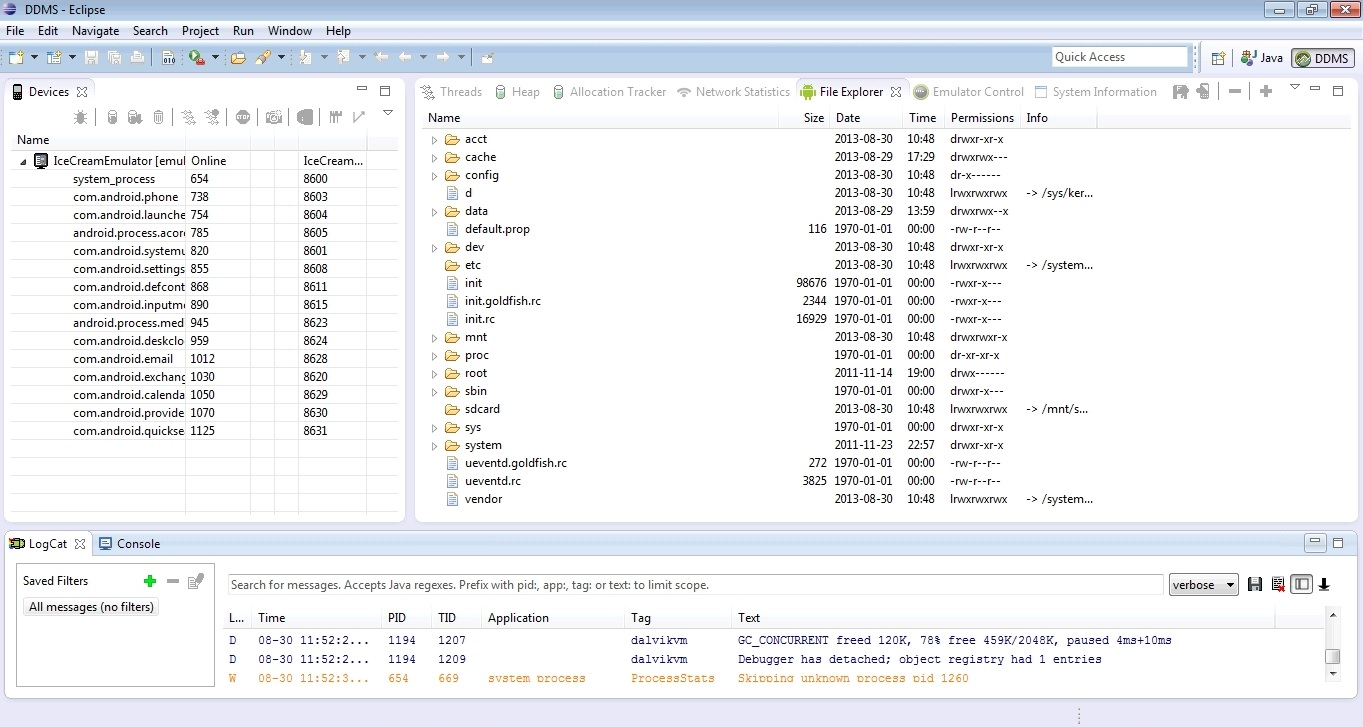
\includegraphics[height=9cm]{images/ddms}
\caption{Στιγμιότυπο του \lt DDMS.\gt}
\label{fig:DDMS}
\end{figure}
To \lt DDMS \gtείναι ένα εργαλείο για \lt debugging \gtτο οποίο περιλαμβάνεται στο \lt Android SDK \gtκαι τρέχει είτε στον \lt emulator \gtείτε σε φυσική κινητή συσκευή. Παρέχει υπηρεσίες \lt port-forwarding \gtκαι καταγραφής συμβάντων \lt (logcat), \gtκαταγράφει στιγμιότυπα της οθόνης της συσκευής, εμφανίζει πληροφορίες για τα νήματα και τον σωρό της συσκευής ενώ προσομοιώνει εισερχόμενες κλήσεις, \lt SMS \gtκαι λήψη σήματος \lt GPS\gt.
\subsection*{Τα εργαλεία πλατφόρμας \lt Android\gt}
\subsection{\lt ADB (Android Debug Bridge)\gt}
Το \lt ADB \gtείναι ένα εργαλείο γραμμής εντολών το οποίο επιτρέπει το \lt debugging \gtτου \lt Android \gtκώδικα μέσω του \lt Eclipse\gt. Το \lt DDMS \gtκαι το \lt ADT \gtχρησιμοποιούν το \lt ADB \gtγια να διευκολύνουν την επικοινωνία του περιβάλλοντος ανάπτυξης και της συσκευής. Ακόμα, το \lt ADB \gtχρησιμοποιείται για την πρόσβαση στο σύστημα αρχείων της συσκευής, την χειροκίνητη εγκατάσταση και την απεγκατάσταση εφαρμογών \lt Android \gtστη συσκευή και την εκτέλεση εντολών φλοιού.
\section{Ανάπτυξη \lt Android \gtΕφαρμογής στο περιβάλλον \lt Eclipse\gt}
\section{Το περιβάλλον \lt Weka\gt}
\subsection{Χρήση του \lt Weka \gtμε κώδικα \lt Java\gt}
\section{Οι χάρτες \lt Google \gtσε περιβάλλον \lt Android\gt}
%%%%%%%%%%%%%%%%%%%%%%%%%%%%%%%%%%%%%%%%%%%%%%%%%%%%%%%%%%%%%%%%%%%%%%%%%%%%%%%%%
%%%%%%%%%%%%%%%%%%%%%%%%%%%%%%%%%%%%%%%%%%%%%%%%%%%%%%%%%%%%%%%%%%%%%%%%%%%%%%%%%
\chapter[Υλοποίηση]{Υλοποίηση}
\label{Chapter6}

%%%%%%%%%%%%%%%%%%%%%%%%%%%%%%%%%%%%%%%%%%%%%%%%%%%%%%%%%%%%%%%%%%%%%%%%%%%%%%%%%
%%%%%%%%%%%%%%%%%%%%%%%%%%%%%%%%%%%%%%%%%%%%%%%%%%%%%%%%%%%%%%%%%%%%%%%%%%%%%%%%%
\chapter[Αποτελέσματα]{Αποτελέσματα}
\label{Chapter6}

%%%%%%%%%%%%%%%%%%%%%%%%%%%%%%%%%%%%%%%%%%%%%%%%%%%%%%%%%%%%%%%%%%%%%%%%%%%%%%%%%
%%%%%%%%%%%%%%%%%%%%%%%%%%%%%%%%%%%%%%%%%%%%%%%%%%%%%%%%%%%%%%%%%%%%%%%%%%%%%%%%%
\chapter[Συμπεράσματα]{Συμπεράσματα}
\label{Chapter6}

\bibliographystyle{plain}
\bibliography{myrefs} 
\addcontentsline{toc}{chapter}{Βιβλιογραφία}

\end{document}


